%% ===========================================================================
%%  Terrain Fine-Detail Blending in Lunar-Landing Simulations
%%  Journal of Automation and Intelligence submission build.
%%  Elsevier CAS bundle, single-column class (cas-sc). To switch to the
%%  double-column typeset layout, change the \documentclass line below to
%%  cas-dc -- the section files under sections/ are class-independent.
%% ===========================================================================
\documentclass[a4paper,fleqn]{cas-sc}

\usepackage[utf8]{inputenc}
\usepackage[T1]{fontenc}
\usepackage{lmodern}
\renewcommand{\ttdefault}{lmtt}

% ---- bibliography: numbered (Vancouver-style) references -----------------
\usepackage[numbers,sort&compress]{natbib}

% ---- math ---------------------------------------------------------------------
\usepackage{mathtools}

% ---- units ------------------------------------------------------------------
\usepackage{siunitx}

% ---- misc -----------------------------------------------------------------
\usepackage{microtype}
\emergencystretch=2em
\usepackage{cleveref}
\crefname{equation}{Eq.}{Eqs.}
\crefname{figure}{Fig.}{Figs.}
\crefname{table}{Table}{Tables}
\crefname{section}{Section}{Sections}

% ---- CAS class tweaks ---------------------------------------------------------
% (a) name the target journal in the first-page footer (default: "Elsevier")
% (b) print the "ORCID(s):" footnote line only when an ORCID is actually given
\ExplSyntaxOn
\cs_set:Npn \__first_footerline:
  {
    \group_begin:
      \small \sffamily
      \ifnum\theblind>0\relax\else \__short_authors: :~ \fi
      { \rmfamily \itshape Journal~of~Automation~and~Intelligence }
    \group_end:
  }
\cs_set:Npn \printorcid
  {
    \seq_if_empty:NF \g_stm_orcid_seq
      {
        \group_begin:
          \tex_let:D \thefootnote \relax \footnotetext
            {
              \raggedright
              \textsc{orcid}(s):\c_space_token
              \seq_use:Nn \g_stm_orcid_seq { ;~ }
            }
        \group_end:
      }
  }
\ExplSyntaxOff

\graphicspath{{figures/}}

\begin{document}
\let\WriteBookmarks\relax
\def\floatpagepagefraction{1}
\def\textpagefraction{.001}

\shorttitle{Terrain fine-detail blending in lunar-landing simulation}
\shortauthors{H. Y. Güloğlu}

\title[mode = title]{Terrain Fine-Detail Blending in Lunar-Landing
Simulations: Comparing Smoothstep, Gaussian, and Hybrid Blending Methods
in Isaac Lab}

\author[1]{Haktan Yusuf Güloğlu}
\cormark[1]
\ead{haktanguloglu24@gmail.com}
\credit{Conceptualization, Methodology, Software, Validation, Formal
analysis, Investigation, Resources, Data curation, Writing -- original
draft, Writing -- review \& editing, Visualization, Supervision, Project
administration}

\affiliation[1]{organization={Sakarya University, National Technology
Workshop, Artificial Intelligence Center},
                city={Sakarya},
                country={Türkiye}}

\cortext[1]{Corresponding author.}

\begin{abstract}
In procedurally generated multi-resolution terrain, the shape of the
blending function joining a coarse global surface to a fine-detail local
patch affects the quality of physically queryable contact geometry, yet
this choice is usually a visual concern, not evaluated quantitatively for
physics fidelity. This study compares the compact-support smoothstep
blend used in a SAC-controlled, gimbal-thrust lunar lander in Isaac Lab
against the infinite-support Gaussian blend inherited from a legacy
codebase, under an equal transition-radius budget, and proposes a hybrid
method using Gaussian blending near the landing-gear contact footprint
and smoothstep beyond it. Across 30 seeds, analytic measurements show the
as-shipped Gaussian produces roughly \num{3200} times worse boundary
height continuity (C0, RMS) and \num{530} times worse slope continuity
(C1) than smoothstep (Wilcoxon signed-rank, $p<\num{1e-8}$), a
scale-invariant defect; a recalibrated Gaussian and the hybrid both
restore near-machine-precision continuity, with negligible VRAM impact.
Isaac Sim training runs (\num{5.73} million steps per method) were first
conducted with a single seed, where the calibrated Gaussian and hybrid
appeared to reach a markedly higher final success rate than smoothstep.
Extending the comparison to two more seeds ($n=3$ total) found no
statistically significant difference between methods on any metric (all
Mann--Whitney $p\ge 0.20$); the apparent gap is largely consistent with
ordinary seed variance. This gives a concrete demonstration of how
misleading single-seed RL comparisons can be: the blend function has a
robust, measurable effect on boundary continuity, but this does not
translate into a distinguishable RL training-performance difference at
the present scale and $n=3$.
\end{abstract}

\begin{highlights}
\item As-shipped Gaussian terrain blending is \textasciitilde\num{3200}x
worse in C0 continuity than smoothstep.
\item A calibrated Gaussian and a new hybrid blend restore near
machine-precision continuity.
\item Single-seed Isaac Sim training seemed to favor Gaussian and hybrid
over smoothstep.
\item Extending to three seeds finds no significant difference among
blends (all $p\ge 0.20$).
\item A concrete case study on how misleading single-seed RL comparisons
can be in practice.
\end{highlights}

% JAI Guide for Authors: maximum of 6 keywords.
\begin{keywords}
Lunar landing simulation \sep Reinforcement learning (Soft Actor-Critic)
\sep Isaac Lab \sep Procedural terrain generation \sep Multi-resolution
blending \sep Continuity analysis
\end{keywords}

\maketitle

\section{Giriş}
\label{sec:giris}

Otonom ay inişi, güç inişi (powered descent) evresinde gerçek zamanlı
olarak kraterli, kayalık ve eğimli bir arazi üzerinde hassas
konumlandırma ve güvenli temas gerektiren, doğrudan operasyonel sonuçları
olan bir kontrol problemidir. Son yıllarda GPU paralel fizik motorları
(NVIDIA PhysX) ve buna dayalı simülasyon çerçeveleri, binlerce ortamı eş
zamanlı çalıştırarak derin pekiştirmeli öğrenmeyle (RL) karmaşık temas
zengini görevlerin pratik sürelerde öğrenilmesini mümkün kılmıştır
\citep{mittal2023orbit,nvidia2025isaaclab,rudin2022walking}. Bu
çalışmanın temelini oluşturan proje de bu sınıfa girer: dört bacaklı, iki
eksenli gimbal itkili bir roketin, Soft Actor-Critic (SAC) algoritmasıyla,
gerçek dijital yükseklik modeli (DEM) tabanlı bir makro yüzey üzerine
bindirilmiş kraterler, kayalar ve santimetre ölçekli regolit dokusuyla
zenginleştirilmiş prosedürel bir ay zemininde inişi öğrendiği bir Isaac
Lab doğrudan iş akışı (direct-workflow) görevidir.

Bu tarz prosedürel çok çözünürlüklü arazilerde, hesaplama ve bellek
bütçesini sınırlı tutmak için tipik olarak iki katman kullanılır: geniş
alanı kapsayan düşük çözünürlüklü bir küresel (global) yüzey ve ajanın ya
da hedefin yakınında yalnızca gerekli bölgede oluşturulan yüksek
çözünürlüklü bir yerel (local) yama. Bu iki katmanın dikişsiz birleşmesi,
bilgisayar grafikleri literatüründe yirmi beş yılı aşkın süredir
çalışılan klasik bir problemdir (geometry clipmaps için
\citep{losasso2004geometry}; ROAM için \citep{duchaineau1997roaming};
geomipmapping için \citep{deboer2000geomipmapping}). Ancak bu literatür
neredeyse tamamen görsel işleme (rendering) kalitesine odaklanır;
birleşme sınırındaki bir süreksizliğin, ayağın zeminle temasını, yükseklik
sensörü okumalarını veya bir RL ajanının proprioseptif gözleminin
gürültü karakterini nasıl etkilediği nicel olarak nadiren ele alınır.

Bu problem, incelenen sistemde iki farklı ve birbiriyle tutarsız çözümle
karşımıza çıkmaktadır: eğitim ortamı katmanlar arasında geçişi kompakt
destekli bir kübik smoothstep fonksiyonuyla sağlarken, önceden kullanılan
mesh tabanlı bir uygulama sonsuz destekli bir Gauss çanı kullanmaktadır.
Bu iki fonksiyon, matematiksel olarak temelden farklı bir özelliğe
sahiptir: smoothstep sonlu bir yarıçapta tam olarak sıfıra iner (kompakt
destek), oysa standart Gauss çanı hiçbir sonlu yarıçapta tam sıfıra
inmez (sonsuz destek; \citep{hardy1971multiquadric}) ve bir mühendislik
uygulamasında kullanılabilmesi için mutlaka bir noktada kesilmesi
(truncation) gerekir; bu kesme işlemi, kesim noktasında yeni ve
ölçülebilir bir dikiş (seam) yaratma riski taşır. Bu iki yöntemi adil
biçimde karşılaştırmak, ikisini de aynı geçiş yarıçapında sıfıra
zorlamayı (hard truncation) ve aynı geçiş bütçesi altında ölçmeyi
gerektirir; bu karşılaştırma biçimi, yapılan literatür taramasında
terrain-randomization çalışmalarının hiçbirinde doğrudan ele alınmamıştır
(bkz. \cref{sec:ilgili}).

Bu gözlemlerden hareketle çalışma üç araştırma sorusuna yanıt aramaktadır:

\begin{itemize}
\item \textbf{AS1:} Kompakt destekli (smoothstep) ve sonsuz destekli
(Gauss) karıştırma fonksiyonları, aynı geçiş yarıçapı bütçesi altında
adil biçimde karşılaştırıldığında, sınır sürekliliği (C0/C1) açısından
nicel olarak ne kadar farklıdır ve bu fark hesaplama/bellek maliyetiyle
nasıl bir denge (trade-off) oluşturur?
\item \textbf{AS2:} İniş ayağı temas bölgesinde Gauss, ötesinde
smoothstep kullanan bir hibrit karıştırma yöntemi, her iki yöntemin
süreklilik avantajlarını makul bir hesaplama maliyeti artışıyla
birleştirebilir mi?
\item \textbf{AS3:} Bu üç karıştırma yönteminin sürekliliğindeki farklar,
gerçek bir Isaac Sim/Isaac Lab SAC eğitiminde ölçülebilir bir öğrenme
performansı farkına yansır mı?
\end{itemize}

Bu doğrultuda çalışmanın amacı üç yönlüdür: (i) mevcut smoothstep
yöntemini ve önceden kullanılan Gauss yöntemini aynı mimaride, aynı
geçiş bütçesi altında nicel olarak karşılaştırmak; (ii) iki yöntemin
avantajlarını birleştiren bir hibrit yöntem önerip doğrulamak; (iii) bu
üç yöntemi yalnızca analitik/CPU düzeyinde değil, gerçek bir Isaac
Sim/Isaac Lab GPU paralel fizik simülasyonu içinde, gerçek bir SAC
eğitimiyle karşılaştırarak, karıştırma fonksiyonu seçiminin öğrenme
performansına yansıyıp yansımadığını göstermektir. Bu son nokta,
çalışmanın özgün değerinin merkezindedir: karşılaştırma soyut bir sayısal
deney olarak değil, gerçek ay zemini üzerinde, gerçek bir Isaac Sim
eğitim döngüsü içinde gerçekleştirilmiştir.

Bu çalışmanın temel katkıları şunlardır:

\begin{itemize}
\item Var olan smoothstep ve önceden kullanılan Gauss karıştırma
yöntemleri, sonlu geçiş yarıçapında kesilerek (hard truncation) aynı
geçiş bütçesi altında ilk kez adil biçimde karşılaştırılmış; kesilmemiş
Gauss'un görünürde iyi durduğu ama gerçekte sonlu yarıçapta kesildiğinde
ortaya çıkan gizli bir dikiş kusuru taşıdığı gösterilmiştir.
\item Temas bölgesinde Gauss, ötesinde smoothstep ağırlıklı bir switch
kullanan yeni bir hibrit karıştırma yöntemi önerilmiş ve bu yöntemin
makine hassasiyetinde süreklilik sağladığı, kendi iç geçişinde yeni bir
dikiş yaratmadığı gösterilmiştir.
\item Otuz tohum ve dört yöntem varyantı (smoothstep, üretim öncesi
Gauss, kalibre edilmiş Gauss, hibrit) üzerinde istatistiksel olarak
doğrulanmış (Wilcoxon işaretli sıra testi) bir süreklilik, maliyet ve
VRAM karşılaştırması yapılmış; dört ayrı ablasyon analiziyle (temas
yarıçapı, switch genişliği, geçiş yarıçapı, grid çözünürlüğü)
bulguların sağlamlığı sınanmıştır.
\item Üç yöntem, gerçek bir Isaac Lab/Isaac Sim PhysX ortamında, GPU
paralel SAC eğitimiyle karşılaştırılmıştır; bu, terrain-randomization
literatüründeki çalışmaların aksine karıştırma fonksiyonu seçimini
doğrudan bir eğitim tasarımı değişkeni olarak ele alan ilk denemedir.
\item Bu gerçek eğitim karşılaştırması yöntem başına tek tohumla değil
üç bağımsız tohumla ($n=3$) yapılmış; ilk tek-tohumlu ölçümde görünen
büyük performans farkının çoklu tohumla istatistiksel olarak
doğrulanamadığı gösterilerek, tek-koşu RL karşılaştırmalarının
güvenilirliği konusunda somut, kendi verisine dayanan bir uyarı örneği
sunulmuştur.
\item Üç yöntem de üretim koduna, mevcut davranışı bozmayan (geriye
dönük uyumlu) ve bir ortam değişkeniyle
(ISAACLAB\_TERRAIN\_BLEND\_METHOD) seçilebilir şekilde entegre
edilmiştir.
\end{itemize}

Bu makalenin geri kalanı şu şekilde yapılandırılmıştır: \cref{sec:ilgili},
çalışmanın konumlandığı literatürü beş tematik küme altında
incelemektedir. \cref{sec:yontem}, deney ortamını ve tüm koşuların
paylaştığı simülasyon kurulumunu, karıştırma fonksiyonlarının matematiksel
tanımını, analitik değerlendirme protokolünü ve gerçek Isaac Sim eğitim
protokolünü ayrıntılandırmaktadır. \cref{sec:bulgular}, süreklilik,
maliyet, VRAM, ablasyon ve gerçek eğitim sonuçlarını sunmaktadır.
\cref{sec:tartisma}, bulguları literatürle ilişkilendirerek tartışmakta ve
sınırlamaları ele almaktadır. \cref{sec:sonuc}, çalışmayı özetlemekte ve
somut gelecek çalışma önerileriyle sonlanmaktadır.

\section{İlgili Çalışmalar}
\label{sec:ilgili}

Bu bölüm, çalışmanın konumlandığı literatürü beş tematik küme altında
incelemektedir. Tarama, hedefli (targeted/scoping) bir kapsam taramasıdır;
PRISMA uyumlu sistematik bir tarama değildir ve her kümede alanın en çok
atıf alan/temel referansları önceliklendirilmiştir.

Küme 1, prosedürel arazide çoklu çözünürlük karıştırma ve LOD (detay
seviyesi) geçişini ele alır. Geometry clipmaps
\citep{losasso2004geometry}, ROAM \citep{duchaineau1997roaming} ve
geomipmapping \citep{deboer2000geomipmapping}, tam olarak bu çalışmanın
iki mesh (küresel + yerel yama) çerçevesinin ait olduğu geleneksel
bilgisayar grafikleri hattını oluşturur; üçü de düşük ve yüksek
çözünürlüklü ağların birleştiği sınırda çatlak/dikiş oluşmasını merkezi
bir mühendislik problemi olarak ele alır. Bu çalışmanın bulgusu, üretim
öncesi Gauss'un sonlu yarıçapta kesildiğinde gerçek bir dikiş bırakması,
bu literatürün yirmi beş yılı aşkın süredir çözmeye çalıştığı aynı sınıf
problemin somut ve ölçülmüş bir örneğidir; smoothstep'in kompakt desteği
ise ROAM ve geoclipmap'in kullandığı sınırda tam sıfıra inen ağırlık
fonksiyonu ilkesiyle örtüşür.

Küme 2, kompakt destekli ve sonsuz destekli karıştırma fonksiyonlarının
süreklilik özelliklerini ele alır. Hardy'nin \citep{hardy1971multiquadric}
topografya için önerdiği multiquadric/Gauss tipi radyal baz fonksiyonu, bu
çalışmadaki üretim öncesi Gauss'un ait olduğu aile gibi sonsuz destekli
olup hiçbir sonlu yarıçapta tam sıfıra inmez; bu, ölçülen kalıntı
davranışıyla (yaklaşık $\exp(-1)\approx\SI{37}{\percent}$) örtüşür.
Wendland \citep{wendland1995piecewise} ise bunun çözümünü formalize eder:
verilen bir düzgünlük derecesi için kompakt destekli, minimal dereceli
pozitif tanımlı radyal fonksiyonlar; smoothstep (kübik Hermite,
\citep{ebert2002texturing}), bu ailenin bir boyutlu, düşük dereceli özel
bir örneğidir. Ohtake ve ark.\ \citep{ohtake2003multiscale}, bu çalışmanın
hibrit yönteminin izlediği stratejiyi tanımlar: kompakt destekli baz
fonksiyonlarla çok ölçekli bir hiyerarşi kurup farklı ölçeklerde farklı
karıştırma davranışı elde etmek.

Küme 3, gezegen/ay inişi simülasyonlarında arazi modelleme ve temas
dinamiğini ele alır. ALHAT programının hedefi
\citep{johnson2008overview,nasajpl_alhat}, yani yüz metre içinde hassas
iniş ve LiDAR tabanlı arazi göreli navigasyon, ve LOLA/SELENE tabanlı
dijital yükseklik modellerinin sunduğu doğruluk düzeyi
\citep{barker2016lunar}, gerçek ay inişi mühendisliğinde arazi
doğruluğunun kozmetik değil doğrudan operasyonel bir gereksinim olduğunu
göstermektedir. Bu, çalışmanın ``neden dikiş/süreklilik önemli''
motivasyonunu güçlendirmektedir: ayak temas bölgesindeki bir süreksizlik,
gerçek ALHAT sınıfı sistemlerde tehlike tespiti ve iniş alanı seçimi
kararlarını etkileyebilecek bir hata sınıfına karşılık gelir. Bu
motivasyon, güncel bir uçuş verisiyle de doğrulanmıştır: JAXA'nın SLIM
görevinin (Ocak 2024) görüş-tabanlı navigasyon ve engel tespiti sonuçları
\citep{ishida2025vision}, inişten \SI{50}{\meter} önce yapılan gerçek
zamanlı engel/arazi tespitinin metre mertebesinde iniş hassasiyeti
sağladığını göstermiş; bu, arazi temsilindeki hataların yalnızca
simülasyonda değil, gerçek uçuşta da doğrudan iniş güvenliğine
yansıdığını somutlaştırmaktadır.

Küme 4, fizik tabanlı RL ortamlarında prosedürel arazi randomizasyonunu
ele alır. Rudin ve ark.\ \citep{rudin2022walking}, IsaacGym üzerinde bu
çalışmadaki terrain havuzuna benzer bir zorluk tabanlı
terrain-curriculum kullanır; bu, çalışmanın curriculum ve terrain-havuzu
tasarımının izole bir örnek olmadığını, alanın yerleşik bir pratiği
olduğunu göstermektedir. Mittal ve ark.\ \citep{mittal2023orbit} (Orbit)
ve NVIDIA \citep{nvidia2025isaaclab} (Isaac Lab), doğrudan bu çalışmanın
kullandığı platformun mimari temelini tanımlarken, Tobin ve ark.\
\citep{tobin2017domain} prosedürel randomizasyonun sim-to-real
transferindeki genel motivasyonu sağlar. Ancak bu kaynakların hiçbiri,
arazi randomizasyonu içindeki çoklu çözünürlük karıştırma fonksiyonunun
kendisini (smoothstep, Gauss veya hibrit) bir tasarım değişkeni olarak
ele almamaktadır; hepsi terrain çeşitliliğine odaklanmakta, blend
şeklinin süreklilik ve öğrenme maliyetine odaklanmamaktadır. Bu çalışma
tam olarak bu boşlukta konumlanmaktadır.

Küme 5, hibrit/bölgesel karıştırma fonksiyonu birleştirmesini (partition
of unity) ele alır. Ohtake ve ark.\ \citep{ohtake2003multiscale}, burada
da merkezi kaynaktır: kompakt destekli baz fonksiyonların çok ölçekli,
partition-of-unity tarzı birleştirilmesi, bu çalışmanın hibrit yönteminin
(temas bölgesinde bir fonksiyon, ötesinde başka bir fonksiyon, aralarında
yumuşak bir switch) genel matematiksel çerçevesidir. Bu çerçeve altında,
hibrit switch'in makine hassasiyetinde yeni bir dikiş yaratmaması
beklenen ve literatürle tutarlı bir sonuçtur: iki C1 düzgün fonksiyonun
C1 düzgün bir ağırlıkla dışbükey birleşimi yine C1 düzgündür.

Özetle, Küme 1 problem sınıfını (çoklu çözünürlük geçişinde
dikiş/süreklilik) sağlarken bu literatür ağırlıklı olarak görsel kaliteye
odaklanmaktadır; bu çalışma aynı problemi fiziksel olarak sorgulanabilir
bir yükseklik alanında (ayak teması) sayısal olarak ölçmektedir. Küme 2,
ampirik bulgunun neden doğru olduğunu elli yılı aşkın bir matematiksel
sonuçla temellendirmektedir; bu bir kodlama hatası değil, radyal baz
fonksiyonlarının bilinen bir yapısal özelliğidir. Küme 3, ``neden
önemli'' sorusuna gerçek dünya mühendislik gerekçesi sağlamaktadır. Küme
4, bu çalışmanın deney platformunun literatürdeki yerini ve doldurduğu
boşluğu netleştirmektedir. Küme 5, önerilen hibrit yöntemi izole bir
mühendislik hilesi olmaktan çıkarıp yerleşik bir matematiksel çerçeveye
oturtmaktadır.

\section{Yöntem}
\label{sec:yontem}

Bu bölüm beş alt bölümden oluşmaktadır: deney ortamı ve görev tanımı, tüm
koşuların paylaştığı simülasyon kurulumu, arazi temsili ve karıştırma
probleminin matematiksel formülasyonu, analitik (CPU) değerlendirme
protokolü ve gerçek Isaac Lab/Isaac Sim eğitim protokolü. Üç karıştırma
yöntemi de önce analitik/CPU düzeyinde, ardından gerçek GPU paralel fizik
simülasyonu içinde aynı sabit geçiş yarıçapı ve aynı hard-truncation
kuralı altında değerlendirilmiştir; bu tutarlılık, iki değerlendirme
katmanı arasındaki bulguların karşılaştırılabilir olmasını sağlamaktadır.

\begin{figure}[t]
\centering
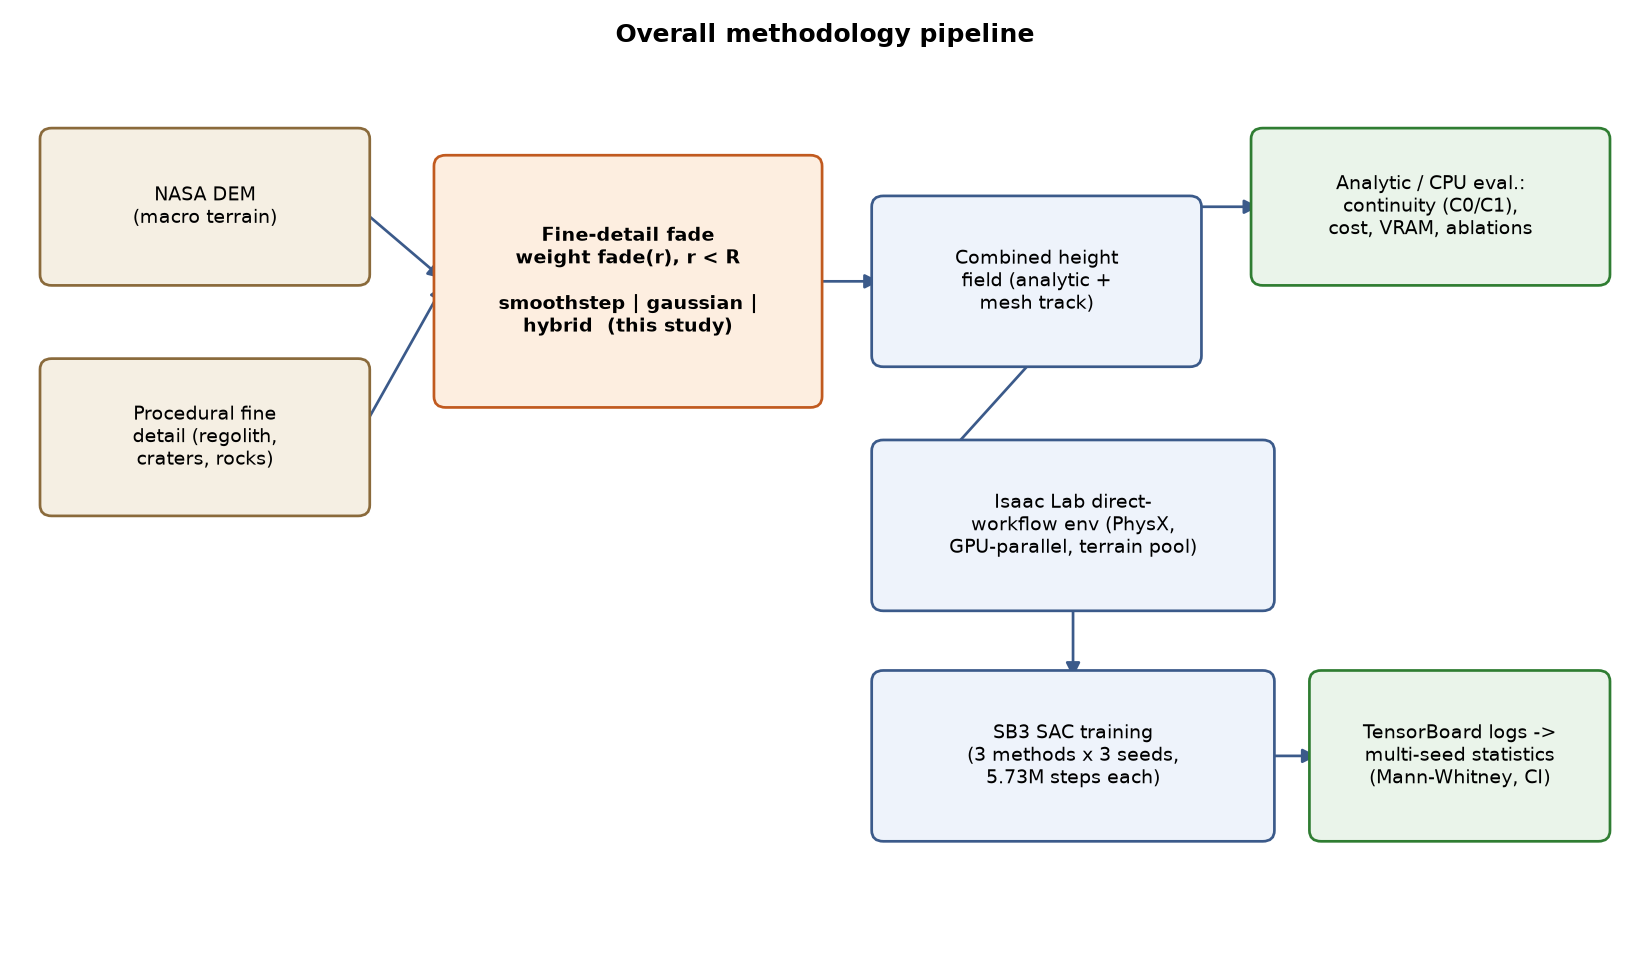
\includegraphics[width=\linewidth]{fig01_methodology.png}
\caption{Genel metodoloji akış şeması: arazi üretiminden (DEM + prosedürel
ince detay), karıştırma fonksiyonu seçimine, analitik/CPU
değerlendirmesine ve gerçek Isaac Lab/SAC eğitim-analiz hattına.}
\label{fig:methodology}
\end{figure}

\subsection{Deney Ortamı ve Görev Tanımı}
\label{sec:ortam}

Deney ortamı, Isaac Lab doğrudan iş akışı (direct-workflow) API'si
üzerinde tanımlanmış bir görev olan \texttt{LunarRocket-Lander-Direct-v0}
'dır. Ajan, dört bacaklı ve iki eksenli gimbal itkili bir roketi temsil
eder; gözlem uzayı konum, hız, yönelim, açısal hız, IMU ve altimetre
okumaları ile hedefe göreli konumu içerir; eylem uzayı ana itki
büyüklüğünü ve gimbal açısını kapsar. Ajan, Stable-Baselines3 (SB3) SAC
(Soft Actor-Critic) algoritmasıyla, NVIDIA PhysX üzerinde GPU paralel
olarak çalışan yüzlerce ortam örneğinde eş zamanlı eğitilmektedir.

Arazi, tek bir prosedürel adımda değil, iki katmanlı bir temsille üretilir:
(i) gerçek bir NASA dijital yükseklik modelinden (DEM) türetilen, rastgele
eğim, krater ve kaya alanlarıyla zenginleştirilmiş bir küresel (global)
makro yüzey; (ii) ajanın başlangıç ve hedef konumlarının yakınında,
santimetre ölçekli çok frekanslı bir gürültü fonksiyonuyla üretilen
yüksek çözünürlüklü bir yerel (local) regolit deseni. Bu iki katman, ortam
sıfırlaması (reset) sırasında arka planda çalışan bir iş parçacığı havuzu
tarafından önceden hazırlanmış bir ``terrain havuzu'' içinden bir yuvanın
(slot) kopyalanmasıyla GPU'ya yüklenir; aktif bölümler (episode) hiçbir
zaman bölüm ortasında değiştirilmez, yeni üretimler yalnızca sıfırlama
anlarında devreye girer. Eğitim, spawn/hedef mesafesi ve komutlanabilir
gimbal yetkisinin, kayan pencereli başarı oranına göre kademeli arttığı
bir müfredat (curriculum) düzeni içinde yürütülmektedir.

Bu iki katmanın birleştiği yerde, yerel yamanın ince detayı, küresel
yüzeye sabit bir yarıçap içinde ``söndürülerek'' (fade) eklenir; bu
söndürme fonksiyonunun matematiksel şekli, bu çalışmanın konusudur ve
\cref{sec:blend}'te tanımlanmaktadır.

\Cref{fig:scene-wide} ve \cref{fig:scene-closeup}, eğitilmiş bir politikanın
gerçek Isaac Lab/Isaac Sim ortamında çalıştırılmasından alınmış, doğrudan
simülasyondan yakalanmış görüntülerdir (offscreen render,
\texttt{ISAACLAB\_CHECKPOINT} ile yüklenen bir kontrol noktası üzerinden;
araç iniş yaklaşımının son evresinde, zemine yaklaşık 0,6--0,7~m
yükseklikteyken yakalanmıştır). Bu yakalama için iki değişiklik
yapılmıştır: (i) sahnenin varsayılan gölgesiz dome light'ı kısılmış ve
düşük açılı, gerçek gölge düşüren yönlü bir ``güneş'' ışığı eklenmiştir,
böylece arazi kabartması ve gölgeler görünür hâle gelmiştir; (ii) iniş
bölgesi, 128x128 küresel yüzeyin yanı sıra 512x512 çözünürlüklü gerçek
yüksek-detay yerel yama (bkz.\ \cref{sec:ortam}, ``yerel regolit deseni'')
ile render edilmiştir, böylece santimetre ölçekli ince doku (toz/kum
taneciği düzeyinde pürüzlülük) da görünür olmuştur. Aracın gerçekten dik
durduğu varsayıma değil, simülasyonun kendi gövde-yönelim verisine
dayanmaktadır: bu koşu boyunca gövdenin yerel yukarı ekseninin dünya $+z$
ekseniyle hizası ($\mathrm{up}_z$) sabit biçimde $+1{,}000$ ölçülmüştür,
yani araç devrilmiş değil, tam dikeydir. \Cref{fig:scene-wide}, dört
bacaklı iniş aracını gerçek kraterli/kayalık ay zemini üzerinde
göstermektedir; sırt hattı, taneli/pürüzlü yüzey dokusu, gölgeler ve
dağınık kayalar, \cref{sec:ortam}'da tanımlanan DEM tabanlı makro
yüzeyin ve prosedürel kaya/krater/ince-detay alanlarının çalışır
durumdaki hâlidir. \Cref{fig:scene-closeup}, aynı karedeki iniş aracının
yakın çekimidir; gövde, iki eksenli gimbal itki ekseninin uçları ve
zeminin taneli dokusu birlikte görülebilmektedir. Bu görüntüler yalnızca
ortamı görsel olarak belgelemek amacıyla sunulmuştur; belirli bir iniş
sonucunu (başarılı/başarısız) temsil ettiği iddia edilmemektedir.

\begin{figure}[t]
\centering
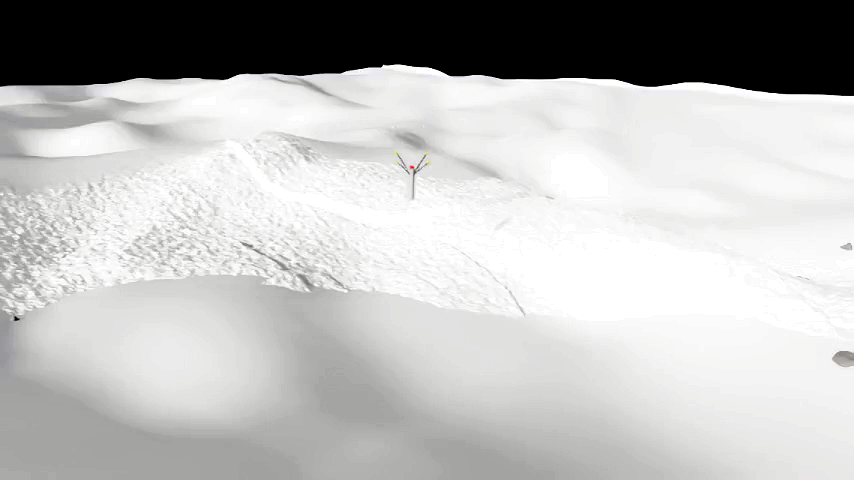
\includegraphics[width=\linewidth]{fig02_scene_wide.png}
\caption{Eğitilmiş politikanın gerçek Isaac Sim ortamında
çalıştırılmasından alınmış sahne görüntüsü: dört bacaklı iniş aracı,
kraterli/kayalık ve taneli dokulu ay zemini üzerinde (yüksek-detay yerel
yama + belgeleme amaçlı yönlü ışık; araç simülasyon verisiyle doğrulanmış
biçimde tam dikeydir, $\mathrm{up}_z=+1{,}000$).}
\label{fig:scene-wide}
\end{figure}

\begin{figure}[t]
\centering
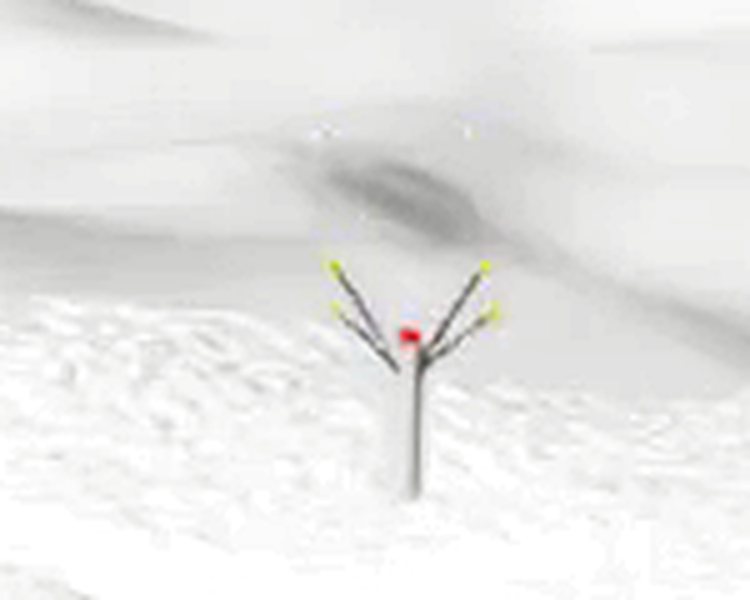
\includegraphics[width=0.6\linewidth]{fig03_scene_closeup.png}
\caption{Aynı sahnenin iniş aracına yakınlaştırılmış görünümü: gövde,
gimbal itki ekseninin uçları ve zeminin santimetre ölçekli taneli dokusu
birlikte görülebilmektedir.}
\label{fig:scene-closeup}
\end{figure}

\subsection{Simülasyon Kurulumu}
\label{sec:simkurulum}

Bu alt bölüm, hem analitik (CPU) protokolün hem de gerçek Isaac
Lab/Isaac Sim eğitim koşularının paylaştığı simülasyon yapılandırmasını
tek bir yerde toplamaktadır (\cref{tab:config}). Fizik, NVIDIA PhysX
üzerinde GPU-paralel olarak $1/120$ saniyelik sabit adımla
(\SI{120}{\hertz}) çözülmekte; politika, \texttt{decimation}~$=2$ ile
\SI{60}{\hertz}'de eylem üretmekte ve her bölüm \SI{20}{\second}, yani
1200 kontrol adımı sürmektedir. Ay yerçekimi
(\SI{1.62}{\meter\per\second\squared}), düşük restitüsyonlu regolit
benzeri bir temas malzemesi ve 512 eş zamanlı ortam örneği tüm koşularda
sabit tutulmuştur.

Araç ve tahrik parametreleri (kütle, itki zarfı, fiziksel ve politika
gimbal limitleri, TVC aktüatör kazançları) ile SAC hiperparametreleri, üç
karıştırma yöntemi arasında değiştirilmemiştir. Yöntemden yönteme değişen
tek büyüklük, \cref{sec:blend}'te tanımlanan ince-detay söndürme
fonksiyonu ve ona bağlı parametrelerdir (\cref{tab:config}'in son grubu;
\texttt{ISAACLAB\_TERRAIN\_BLEND\_METHOD} ortam değişkeniyle seçilir). Bu
sabitleme, \cref{sec:bulgular}'da gözlemlenen farkların yalnızca
karıştırma yöntemine atfedilebilmesi için gereklidir.

Gerçek eğitim karşılaştırması, hesaplama bütçesi kısıtı nedeniyle tam
ölçekli (1200 iterasyon) yapılandırmanın kısaltılmış bir versiyonuyla
-yöntem başına üç bağımsız tohum, koşu başına yaklaşık 5,73 milyon ortam
adımı- yürütülmüştür; bu ölçek sınırlaması \cref{sec:egitimprotokolu} ve
\cref{sec:egitimsonuclari}'te ayrıca ele alınmaktadır.

\begin{table}[t]
\centering
\caption{Analitik protokol ile gerçek Isaac Lab/Isaac Sim eğitim
koşularının paylaştığı simülasyon, araç, RL eğitim ve arazi karıştırma
parametreleri. Yalnızca son grup (karıştırma parametreleri), yöntemden
yönteme değişir.}
\label{tab:config}
\footnotesize
\begin{tabular}{@{}p{0.19\linewidth}p{0.33\linewidth}p{0.38\linewidth}@{}}
\toprule
\textbf{Grup} & \textbf{Parametre} & \textbf{Değer} \\
\midrule
\multirow{10}{*}{Fizik / simülasyon}
 & Fizik motoru & NVIDIA PhysX 5 (GPU ardışık düzeni) \\
 & Simülasyon adımı (dt) & $1/120$~s (\SI{120}{\hertz}) \\
 & Kontrol frekansı (decimation = 2) & \SI{60}{\hertz} \\
 & Bölüm süresi & \SI{20}{\second} (1200 kontrol adımı) \\
 & Yerçekimi & $0,0,-1.62$~m/s$^2$ \\
 & Paralel ortam sayısı & 512 \\
 & Ortam aralığı (env\_spacing) & \SI{90}{\meter} \\
 & Fizik kopyalama & replicate\_physics + clone\_in\_fabric (açık) \\
 & Sürtünme (statik / dinamik) & 0.85 / 0.65 (combine: multiply) \\
 & Restitüsyon & 0.02 \\
\midrule
\multirow{9}{*}{Araç ve tahrik}
 & Araç kütlesi & 1.66~kg (1.63 gövde + gimbal bağlantıları) \\
 & Maksimum itki & 30~N \\
 & Maksimum komut throttle & 0.35 ($\approx$~10.5~N etkin) \\
 & Fiziksel gimbal limiti & $\pm25^\circ$ (mekanik sert durdurucu) \\
 & Politika gimbal zarfı & $4^\circ$--$8^\circ$ (müfredat zorluğuyla ölçeklenir) \\
 & İtki kaldıraç kolu & 0.25~m \\
 & TVC aktüatör (implicit) & effort 2.5, stiffness 10, damping 0.1, armature 0.002 \\
 & Gözlem / eylem boyutu & 125 / 3 \\
 & Başlangıç irtifası & 25~m (dik yönelim) \\
\midrule
\multirow{12}{*}{RL eğitimi (SB3 SAC)}
 & Politika ağı & MLP [384, 256, 128], ELU \\
 & Replay buffer & 1\,000\,000 \\
 & learning\_starts & 16\,384 \\
 & Batch boyutu & 1024 \\
 & Öğrenme oranı & $3\times10^{-4}$ \\
 & $\gamma$ / $\tau$ & 0.99 / 0.005 \\
 & train\_freq / gradient\_steps & 1 / 32 \\
 & Entropi katsayısı & otomatik (target\_entropy = $-1.5$) \\
 & Normalizasyon & normalize\_input + normalize\_value açık, clip\_obs = 10 \\
 & Karşılaştırma bütçesi & 350 iter $\times$ 32 $\times$ 512 $\approx$ 5.73~M ortam adımı \\
 & Tohumlar & 42, 7, 123 (yöntem başına $n=3$, ardışık) \\
 & Cihaz & tek GPU (cuda:0) \\
\midrule
\multirow{9}{*}{Karıştırma parametreleri}
 & Geçiş yarıçapı ($R$) & 8.0~m \\
 & Yöntem seçenekleri & smoothstep / gaussian / hybrid (ISAACLAB\_TERRAIN\_BLEND\_METHOD) \\
 & Kalibre Gauss katsayısı ($k$) & $\ln(1000)\approx 6.9078$ \\
 & Hibrit temas yarıçapı ($r_c$) & 1.5~m \\
 & Hibrit switch genişliği ($w$) & 0.3~m \\
 & İnce-detay genlik aralığı & 0.006--0.020~m \\
 & Makro yükseklik / eğim ölçeği & 0.45~m / 0.035 \\
 & Krater / kaya sayısı (bölüm başına) & 3 / 5 \\
 & Terrain havuzu (boyut / yenileme) & 15 yuva / 60 atama \\
\bottomrule
\end{tabular}
\end{table}

\subsection{Arazi Temsili ve Karıştırma Fonksiyonları}
\label{sec:blend}

Yerel yamanın ince detay yüksekliği, küresel yüzeye üç aday söndürme
(fade) fonksiyonundan biriyle eklenir. Her üç fonksiyon da $r$ merkezden
uzaklık ve $R=\texttt{terrain\_detail\_radius\_m}=8{,}0$~m sabit geçiş
yarıçapı olmak üzere $r\ge R$ için tam olarak sıfıra zorlanır (hard
truncation); bu, üç yöntemi aynı geçiş bütçesi altında karşılaştırılabilir
kılan temel metodolojik düzenlemedir ve üretim kodunda da bu şekilde
uygulanmaktadır.

\textbf{Smoothstep} (kompakt destek, varsayılan/mevcut yöntem): $t =
\mathrm{clamp}(1-r/R,\,0,\,1)$ olmak üzere
\begin{equation}
\mathrm{fade}(r) = t^2\,(3-2t).
\label{eq:smoothstep}
\end{equation}
Bu fonksiyon $r=R$'de zaten tam olarak sıfırdır; ek bir kesme adımına
ihtiyaç duymaz ve C1 sürekliliği analitik olarak garantidir.

\textbf{Gauss} (sonsuz destek, önceden kullanılan yöntem):
\begin{equation}
\mathrm{fade}(r) = \exp\!\left(-k\,(r/R)^2\right).
\label{eq:gauss}
\end{equation}
Bu çalışmada iki $k$ değeri ayrı ayrı değerlendirilmiştir: önceden
kullanılan (as-shipped) sabit $k=1{,}0$ ve bu çalışmada önerilen, Gauss'un
pratik desteğinin $R$'de yaklaşık binde bir düzeyine inmesini sağlayan
kalibre edilmiş sabit $k=\ln(1000)\approx 6{,}9078$. Üretim kodundaki
\texttt{cfg.terrain\_gaussian\_k} alanı, varsayılan olarak kalibre
edilmiş sabiti kullanır; üretim öncesi $k=1{,}0$ yalnızca bu çalışmanın
analitik/CPU karşılaştırmasında, mevcut kusuru göstermek amacıyla ayrı
bir varyant (\texttt{gaussian\_shipped}) olarak test edilmiştir. Her iki
$k$ değeri için de fonksiyon, $r\ge R$'de dışarıdan sıfıra zorlanır.

\textbf{Hibrit} (önerilen yöntem): İniş ayağı temas izi yarıçapı $r_c =
\texttt{terrain\_hybrid\_contact\_radius\_m}=1{,}5$~m ve switch genişliği
$w=\texttt{terrain\_hybrid\_switch\_width\_m}=0{,}3$~m olmak üzere,
$[r_c-w/2,\,r_c+w/2]$ aralığında smoothstep ağırlıklı bir $\mathrm{switch}(r)$
tanımlanır:
\begin{equation}
u = \mathrm{clamp}\!\left(\frac{\mathrm{hi}-r}{\mathrm{hi}-\mathrm{lo}},\,0,\,1\right),
\qquad
\mathrm{switch}(r) = u^2\,(3-2u),
\label{eq:switch}
\end{equation}
burada $\mathrm{lo}=r_c-w/2$, $\mathrm{hi}=r_c+w/2$. Nihai söndürme,
\begin{equation}
\mathrm{fade}(r) = \mathrm{switch}(r)\cdot\mathrm{gauss}(r) +
\left(1-\mathrm{switch}(r)\right)\cdot\mathrm{smoothstep}(r)
\label{eq:hybrid}
\end{equation}
olarak tanımlanır; yani ayak temas bölgesine yakın kısımda ağırlıklı
olarak Gauss, ötesinde ağırlıklı olarak smoothstep kullanılır ve iki
fonksiyon arasındaki geçiş, kendisi de C1 düzgün olan bir smoothstep
ağırlıkla yumuşatılır. $r=R$ sınırında $\mathrm{switch}(r)=0$ olduğundan,
hibrit yöntem bu sınırda analitik olarak smoothstep ile birebir aynıdır.

Bu üç yöntem, üretim kodunda \texttt{ISAACLAB\_TERRAIN\_BLEND\_METHOD}
ortam değişkeniyle (\texttt{smoothstep} \textbar\ \texttt{gaussian}
\textbar\ \texttt{hybrid}) seçilebilir şekilde, mevcut varsayılan
davranışı (smoothstep) değiştirmeden entegre edilmiştir.

\subsection{Analitik (CPU) Değerlendirme Protokolü}
\label{sec:analitikprotokol}

Analitik değerlendirme, Isaac Lab/torch bağımlılığı olmadan, üretim
kodundaki formüllerin bire bir NumPy taşıması üzerinde, iki bağımsız
izleme (track) ile yürütülmüştür: (i) mesh-track, gerçek üçgen ağı üretip
vertex sayısı ve süre ölçen bir izleme; (ii) analytic-track, yükseklik
alanını doğrudan sürekli bir fonksiyon olarak sorgulayan bir izleme. İki
izlemenin birbirini doğrulaması, bulguların mesh ayrıklaştırmasına özgü
bir yapay etki olmadığını göstermek için kullanılmıştır.

Süreklilik metrikleri, sonlu farklarla hesaplanmıştır: C0 (yükseklik)
sürekliliği, geçiş sınırının hemen iki tarafındaki noktalar arasındaki
yükseklik farkının mutlak değeri (uzamsal epsilon = 0,05~m); C1 (eğim)
sürekliliği, aynı noktalardaki yerel gradyanın açısal farkı (gradyan
epsilon = 0,02~m) olarak tanımlanmıştır. Ölçümler 720 açısal örnek
üzerinden alınmış ve hem maksimum hem RMS (kök ortalama kare) değerleri
raporlanmıştır. İlk ölçümlerde, birleşik (küresel + yerel) yükseklik
üzerinden yapılan ölçümün, doğal arazi eğiminin epsilon aralığındaki
varyasyonuyla karışarak asıl dikiş sinyalini bastırdığı görülmüş; bu
nedenle yalnızca söndürülmüş ince detay bileşenini
($\mathrm{fade}(r)\cdot\mathrm{ince\_detay}(x,y)$) izole eden bir
``detail-only'' ölçüm modu tanımlanmış ve bu, çalışmanın başlık
(headline) metriği olarak benimsenmiştir; birleşik yüzey üzerindeki ölçüm
ikincil/gerçekçi bir referans olarak korunmuştur.

Bellek maliyeti, vertex başına 32 bayt ve çarpışma (collision) ağı için
2x çarpan varsayımıyla, iki-mesh (literal, ayrı küresel ve yerel ağlar)
ile tek-grid (baked, tek birleşik ağ) muhasebe biçimleri için ayrı ayrı
tahmin edilmiştir. Sorgu verimi (throughput), 512 ortam ve ortam başına
64 küresel + 24 yerel + 4 ince-detay sorgusu (toplam 92 sorgu/ortam)
varsayımıyla, saf söndürme formülünün (fade-only, terrain örneklemesinden
izole) mikro-saniye cinsinden maliyeti ayrıca ölçülmüştür.

Ana karşılaştırma, dört yöntem varyantı (smoothstep, üretim öncesi Gauss,
kalibre edilmiş Gauss, hibrit) için otuz bağımsız rastgele tohum
üzerinde tekrarlanmıştır; istatistiksel anlamlılık, her tohumda
hesaplanan $\log_{10}$ oran farkları üzerinde Wilcoxon işaretli sıra
testiyle değerlendirilmiştir (parametrik testler yerine bu test tercih
edilmiştir, çünkü bazı karşılaştırmalarda -örneğin hibrit ile
smoothstep, $r=R$'de analitik olarak özdeş olduğundan- fark dağılımı
sıfır varyansa yakınsamakta ve Cohen's $d$ gibi parametrik büyüklük
ölçütleri yozlaşmaktadır).

Bulguların sağlamlığı dört ayrı ablasyon analiziyle sınanmıştır: (i)
temas yarıçapı ($r_c$) taraması, 1,0--4,0~m aralığında; (ii) switch
genişliği ($w$) taraması, 0,05--2,0~m aralığında; (iii) geçiş yarıçapı
($R$) taraması, 4--16~m aralığında, kusurun ölçek değişmezliğini test
etmek için; (iv) grid çözünürlüğü taraması, yaklaşık 0,31--1,27~m grid
aralığı üzerinde, log-log doğrusal regresyonla ampirik yakınsama derecesi
(convergence order) tahmin edilerek.

\subsection{Gerçek Isaac Lab/Isaac Sim Eğitim Protokolü}
\label{sec:egitimprotokolu}

Analitik değerlendirmenin ardından, üç yöntem (smoothstep, kalibre
edilmiş Gauss, hibrit) gerçek bir Isaac Lab/Isaac Sim eğitim ortamında
karşılaştırılmıştır. Bu, çalışmanın özgün değerinin merkezini
oluşturur: karşılaştırma soyut bir sayısal deney olarak değil, gerçek
kraterli/eğimli ay zemini üzerinde, GPU paralel PhysX fizik simülasyonu
içinde çalışan bir SAC eğitim döngüsüyle gerçekleştirilmiştir.

Her yöntem, \texttt{ISAACLAB\_TERRAIN\_BLEND\_METHOD} ortam değişkeniyle
seçilerek, aynı donanımda (tek makine, tek GPU), aynı hiperparametre
yapılandırmasıyla (\texttt{sb3\_sac\_cfg.yaml}) ve GPU/VRAM çakışmasını
önlemek amacıyla eş zamanlı değil ardışık olarak eğitilmiştir. Her koşu
5.734.400 ortam adımı (yaklaşık 350 iterasyon) sürmüştür; bu, hesaplama
bütçesi kısıtı nedeniyle tam ölçekli (1200 iterasyon) yapılandırmanın
kısaltılmış ama anlamlı bir sinyal verecek şekilde küçültülmüş bir
versiyonudur ve bu, çalışmanın açıkça belirtilmesi gereken bir ölçek
sınırlamasıdır.

İlk ölçüm, SAC ajanının yapılandırma dosyasındaki varsayılan tohumla
(seed~$=42$) yöntem başına tek koşu olarak yapılmıştır. Bu tek-koşu
tasarımının Henderson ve ark.'nın \citep{henderson2018deep} uyardığı
türden bir tuzak olduğu göz önünde bulundurularak, çalışma iki ek
bağımsız tohumla (seed~$=7$ ve seed~$=123$) genişletilmiş ve her yöntem
için toplam üç bağımsız koşu ($n=3$) elde edilmiştir
-\texttt{ISAACLAB\_SEED} ortam değişkeni bu amaçla üretim koduna
eklenmiştir. GPU paralel PhysX fizik simülasyonunun kendi içsel
belirlenimsizliği (iş parçacığı zamanlaması, kayan nokta indirgeme
sırası) ve terrain havuzunun arka planda çalışan CPU üretim sürecinin
zamanlamaya bağlı olması nedeniyle, aynı tohumla bile iki koşu birbirinin
bit eşdeğeri tekrarı değildir; dolayısıyla üç tohum, ajan başlatma
kaynaklı varyansın yanı sıra bu sistem-düzeyi belirlenimsizliği de
örnekler.

Eğitim metrikleri (başarı oranı, zaman aşımı oranı, sert iniş oranı,
müfredat zorluğu, entropi katsayısı, xy-ilerleme ödülü) TensorBoard
üzerinden loglanmış ve olay dosyaları (event files)
\texttt{tensorboard.backend.event\_processing.EventAccumulator} ile
ayrıştırılmıştır. Her (yöntem, tohum) koşusu için nihai performans, o
koşunun son yüzde onluk penceresindeki loglanmış noktaların ortalaması
alınarak TEK bir özet değere indirgenmiştir; yöntemler arası
karşılaştırmalar bu üç bağımsız özet değer üzerinde (bağımsız örneklem
olarak) Mann-Whitney U testi ve 5000 tekrarlı bootstrap \%95 güven
aralığı ile yapılmıştır. Bu, bir tek koşunun içindeki otokorelasyonlu
(bağımsız olmayan) noktaları sahte-bağımsız örneklem gibi kullanmaktan
(pseudoreplication) kaçınan, istatistiksel olarak doğru birimdir; ancak
$n=3$ ile istatistiksel güç düşüktür ve bu husus \cref{sec:egitimsonuclari}
ve \cref{sec:tartisma}'te açıkça vurgulanmaktadır.

\section{Bulgular}
\label{sec:bulgular}

Bu bölüm, sınır sürekliliği ve hesaplama maliyeti bulgularını, ardından
dört ablasyon analizinin sonuçlarını ve son olarak gerçek Isaac Sim
eğitim karşılaştırmasının sonuçlarını sunmaktadır. Yöntem tekrarı
yapılmamış, veri/deney tasarımı ayrıntıları \cref{sec:yontem}'e
bırakılmıştır.

\subsection{Sınır Sürekliliği ve Hesaplama Maliyeti}
\label{sec:sureklilik}

\Cref{tab:continuity}, otuz tohum üzerinde toplanmış (aggregated),
yalnızca söndürülmüş ince detay bileşenini izole eden başlık (headline)
süreklilik ölçümlerini, smoothstep'e göre oran olarak özetlemektedir.
Üretim öncesi Gauss (\texttt{gaussian\_shipped}, $k=1{,}0$), smoothstep'e
kıyasla ortalama 3192 kat daha kötü C0 (yükseklik) sürekliliği ve 535 kat
daha kötü C1 (eğim) sürekliliği üretmektedir; her iki fark da Wilcoxon
işaretli sıra testiyle son derece anlamlıdır ($p=1{,}86\times10^{-9}$,
$n=30$). Kalibre edilmiş Gauss ($k=\ln(1000)$), bu kusuru büyük ölçüde
gidermekte, ancak yine de smoothstep'e göre ölçülebilir düzeyde (C0'da
yaklaşık 9,3 kat, C1'de yaklaşık 1,6 kat) daha yüksek kalıntı hata
bırakmaktadır. Hibrit yöntem, $r=R$ sınırında analitik olarak smoothstep
ile birebir aynı olduğundan ($\mathrm{switch}(R)=0$), otuz tohumun
tamamında sıfır fark göstermiştir; bu, bir ölçüm sonucu değil, yöntemin
tanımından kaynaklanan beklenen bir sonuçtur.

\begin{table}[t]
\centering
\caption{Otuz tohum üzerinde toplanmış, yalnızca ince-detay bileşenini
izole eden sınır sürekliliği oranları (smoothstep'e göre).}
\label{tab:continuity}
\footnotesize
\begin{tabular}{@{}lccc c@{}}
\toprule
\textbf{Method} & \textbf{C0 oranı} & \textbf{C1 oranı} & \textbf{Wilcoxon $p$} & \textbf{$n$ (seed)} \\
\midrule
smoothstep (referans) & 1.0 & 1.0 & -- & 30 \\
gaussian\_shipped ($k$=1.0) & 3192x & 535x & 1.86e-09 & 30 \\
gaussian\_calibrated ($k$=ln(1000)) & 9.3x & 1.6x & 1.86e-09 & 30 \\
hybrid & 1.0 (özdeş) & 1.0 (özdeş) & n/a (analitik olarak özdeş) & 30 \\
\bottomrule
\end{tabular}
\end{table}

\Cref{fig:radial-profile}, dört yöntem varyantının birleşik (makro + ince
detay) yükseklik kesitini göstermektedir. Bu ölçekte dört eğri neredeyse
tam olarak üst üste binmektedir, çünkü ince detay genliği (santimetre
mertebesinde) makro arazi ölçeğine (metre mertebesinde) kıyasla çok
küçüktür; \cref{tab:continuity}'de raporlanan büyüklük mertebesindeki
farklar bu görsel ölçekte çıplak gözle seçilemez. Bu,
\cref{sec:analitikprotokol}'te tanımlanan ``detail-only'' izolasyon
adımının neden gerekli olduğunu doğrudan göstermektedir: dikiş kusuru,
yalnızca ince detay bileşeni ayrıştırıldığında ortaya çıkmaktadır.

\begin{figure}[t]
\centering
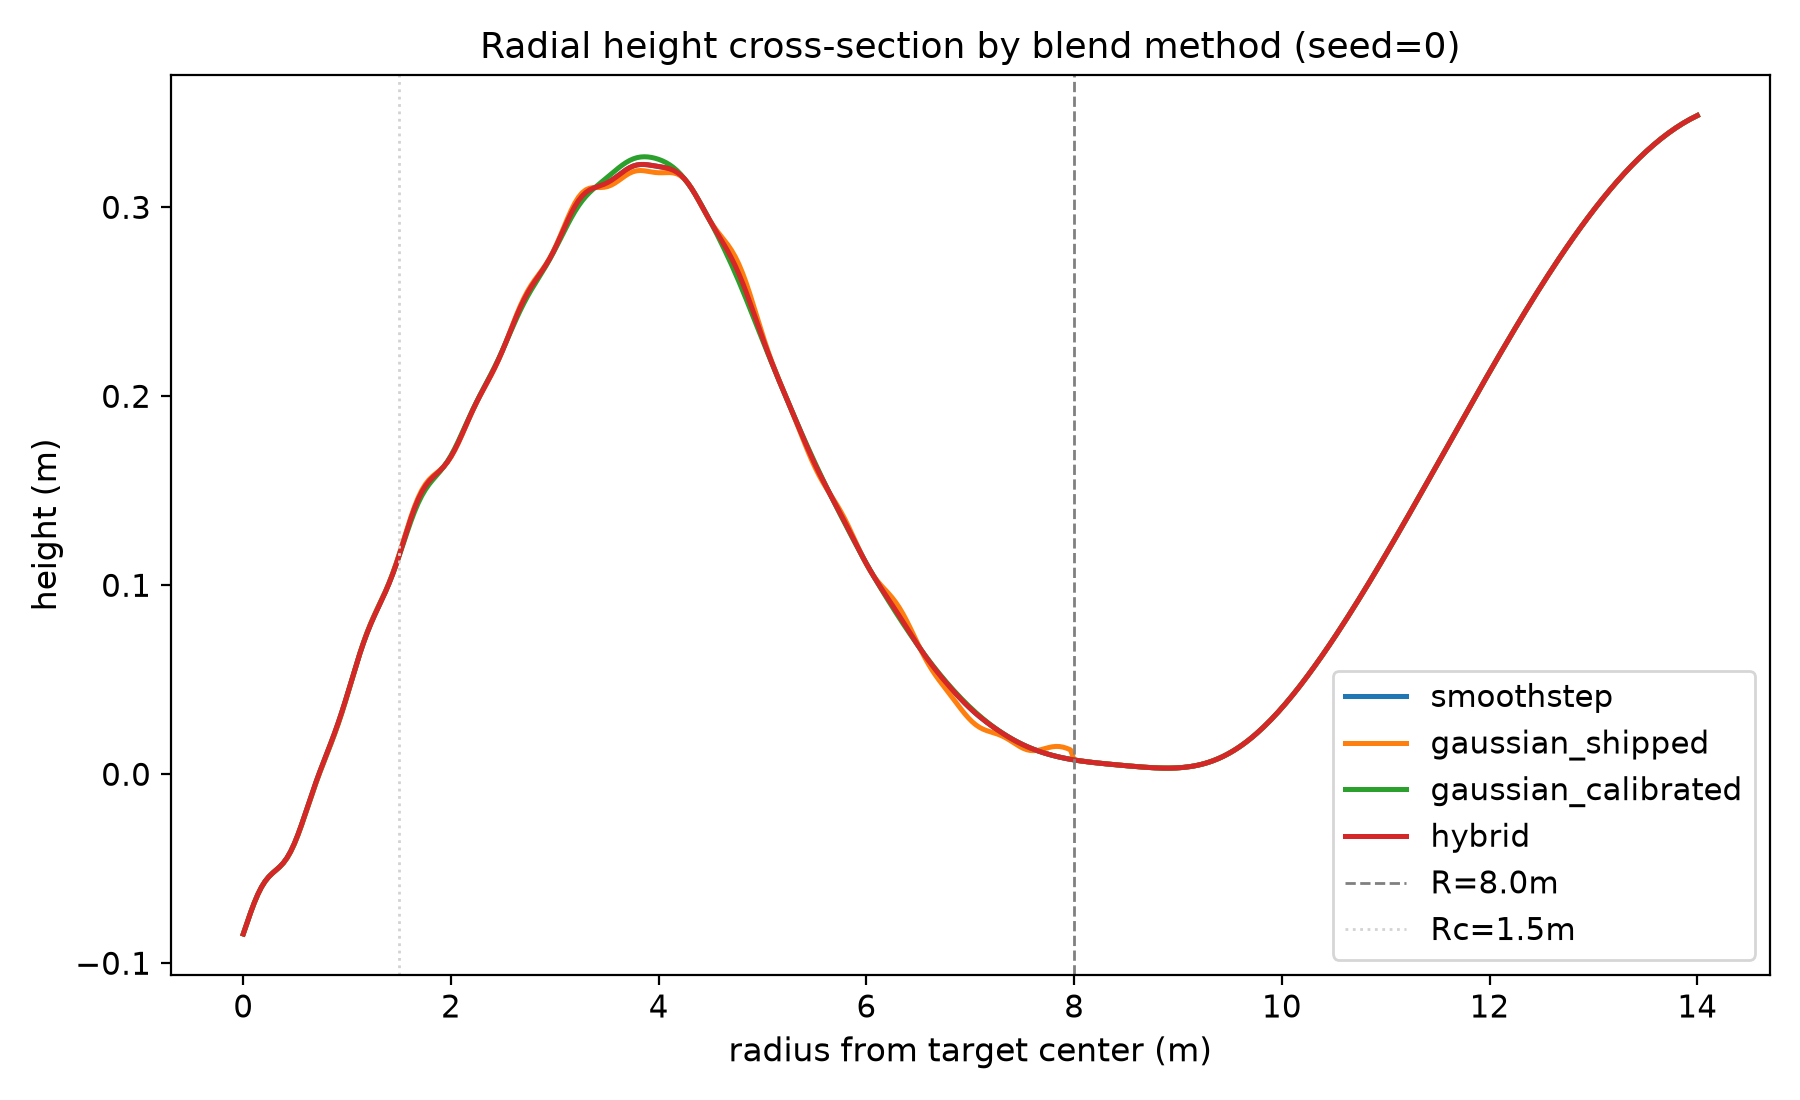
\includegraphics[width=\linewidth]{fig04_radial_profile.png}
\caption{Üç karıştırma yönteminin radyal söndürme profili.}
\label{fig:radial-profile}
\end{figure}

\Cref{tab:cost}, yalnızca söndürme formülünün kendisinin (arazi
örneklemesinden izole) mikro-saniye cinsinden hesaplama maliyetini
göstermektedir. Smoothstep en düşük maliyete sahiptir (93,1
mikrosaniye); Gauss varyantları (üretim öncesi ve kalibre edilmiş)
benzer, orta düzey bir maliyete sahiptir (yaklaşık 149--150 mikrosaniye);
hibrit yöntem ise en yüksek maliyete sahiptir (407,8 mikrosaniye,
smoothstep'in yaklaşık 4,3 katı), çünkü her sorguda hem Gauss hem
smoothstep dallarını hem de switch ağırlığını hesaplamaktadır.

\begin{table}[t]
\centering
\caption{Söndürme (fade) formülünün sorgu başına hesaplama maliyeti.}
\label{tab:cost}
\begin{tabular}{@{}lc@{}}
\toprule
\textbf{Method} & \textbf{Cost (\si{\micro\second}/query)} \\
\midrule
smoothstep & 93.12 \\
gaussian\_shipped & 148.84 \\
gaussian\_calibrated & 149.61 \\
hybrid & 407.83 \\
\bottomrule
\end{tabular}
\end{table}

\Cref{fig:continuity-bars}, \cref{tab:continuity}'deki analitik ve
mesh-track süreklilik ölçümlerini yöntem başına çubuk grafik olarak
görselleştirmektedir; \texttt{gaussian\_shipped}'in dört panelin
tamamında diğer üç yönteme kıyasla düzenlerce daha yüksek hata çubuğuna
sahip olması, tabloda raporlanan büyüklük farkını görsel olarak da
doğrulamaktadır.

\begin{figure}[t]
\centering
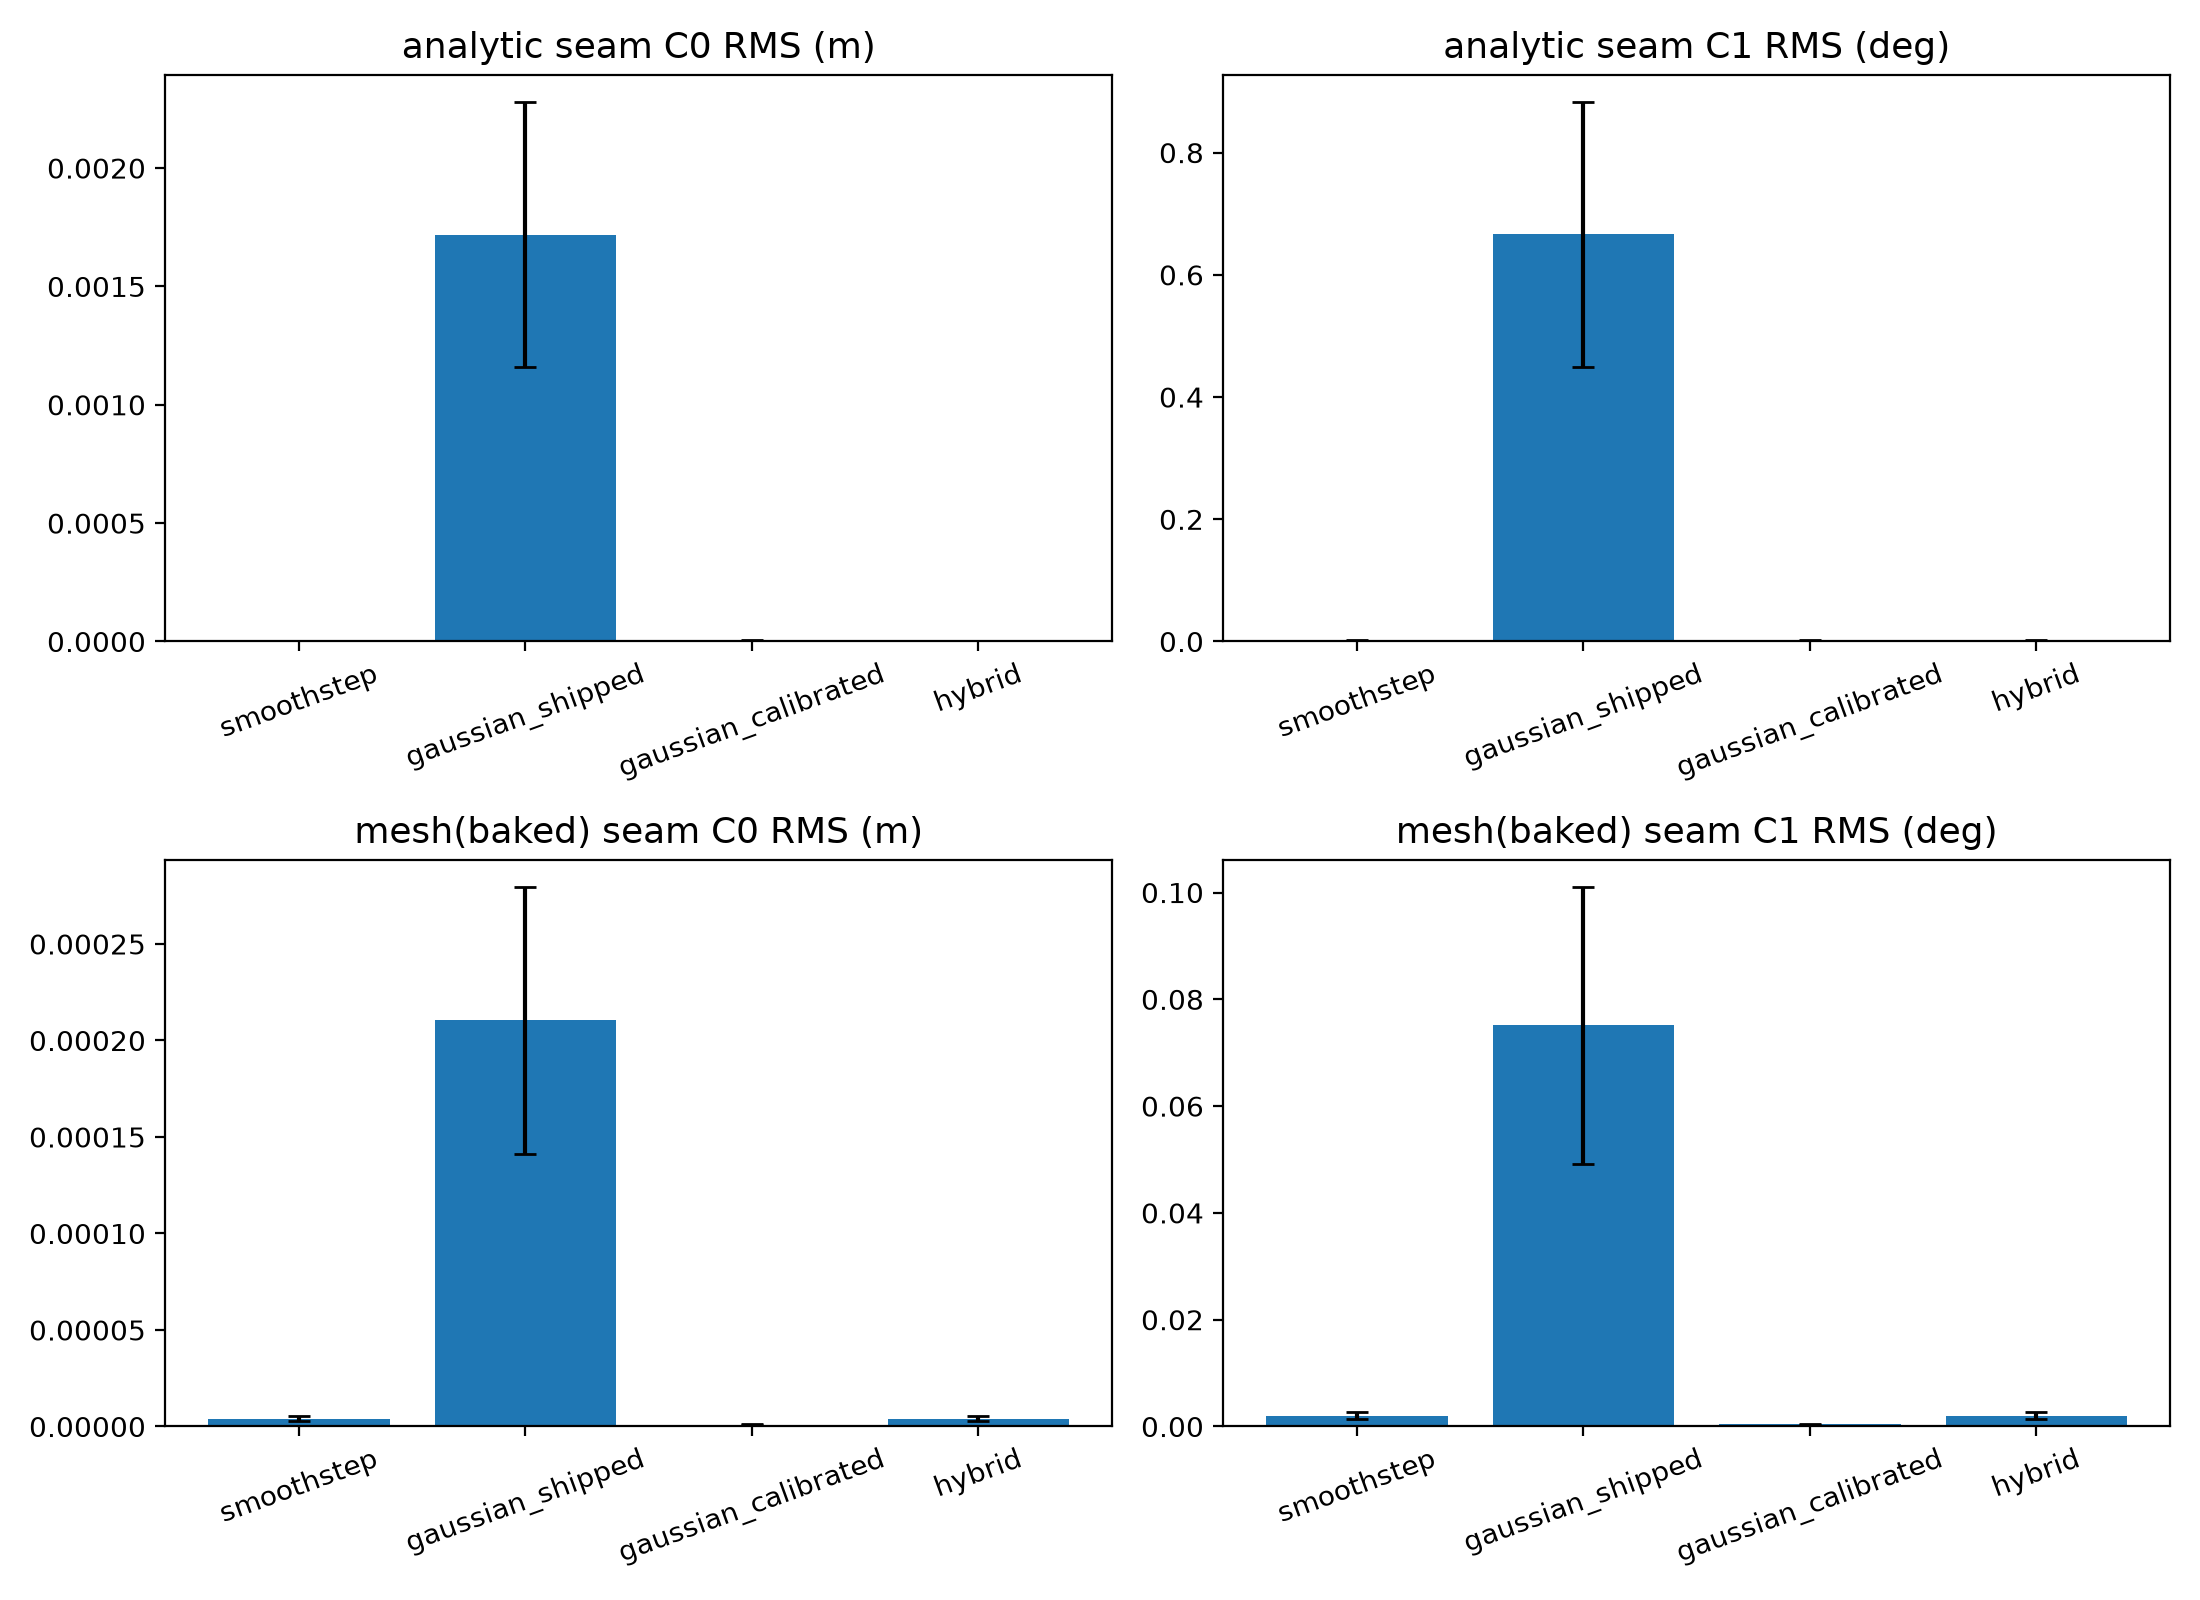
\includegraphics[width=\linewidth]{fig05_continuity_bars.png}
\caption{Yöntemler arası C0/C1 sınır sürekliliği karşılaştırması.}
\label{fig:continuity-bars}
\end{figure}

\Cref{tab:vram}, iki mesh muhasebe biçimi için bellek tahminini
göstermektedir; bu tahmin yalnızca ağ geometrisine (vertex sayısı)
bağlıdır ve karıştırma yönteminin şekli VRAM üzerinde ölçülebilir bir
etki yaratmamaktadır -gerçek VRAM kaldıracı, karıştırma fonksiyonu
seçimi değil, ağ topolojisi tercihidir (iki-mesh'e karşı tek-grid).

\begin{table}[t]
\centering
\caption{Ağ muhasebe biçimine göre tahmini VRAM kullanımı.}
\label{tab:vram}
\begin{tabular}{@{}lc@{}}
\toprule
\textbf{Mesh accounting scheme} & \textbf{Estimated memory (MB)} \\
\midrule
Two-mesh (literal: separate global + local meshes) & 5.24 \\
Single-grid (baked: one combined mesh) & 1.05 \\
\bottomrule
\end{tabular}
\end{table}

\Cref{fig:cost-comparison}, \cref{tab:cost} ve \cref{tab:vram}'teki maliyet
ölçütlerini tek bir görünümde birleştirmektedir: mesh-track üretim
süresi ve analytic-track sorgu verimi yöntemler arasında görece
yakınken, hibrit'in fade-only maliyetteki belirgin sıçraması ve dört
yöntemin de aynı VRAM ayak izini paylaştığı aynı grafik takımında bir
arada görülebilmektedir.

\begin{figure}[t]
\centering
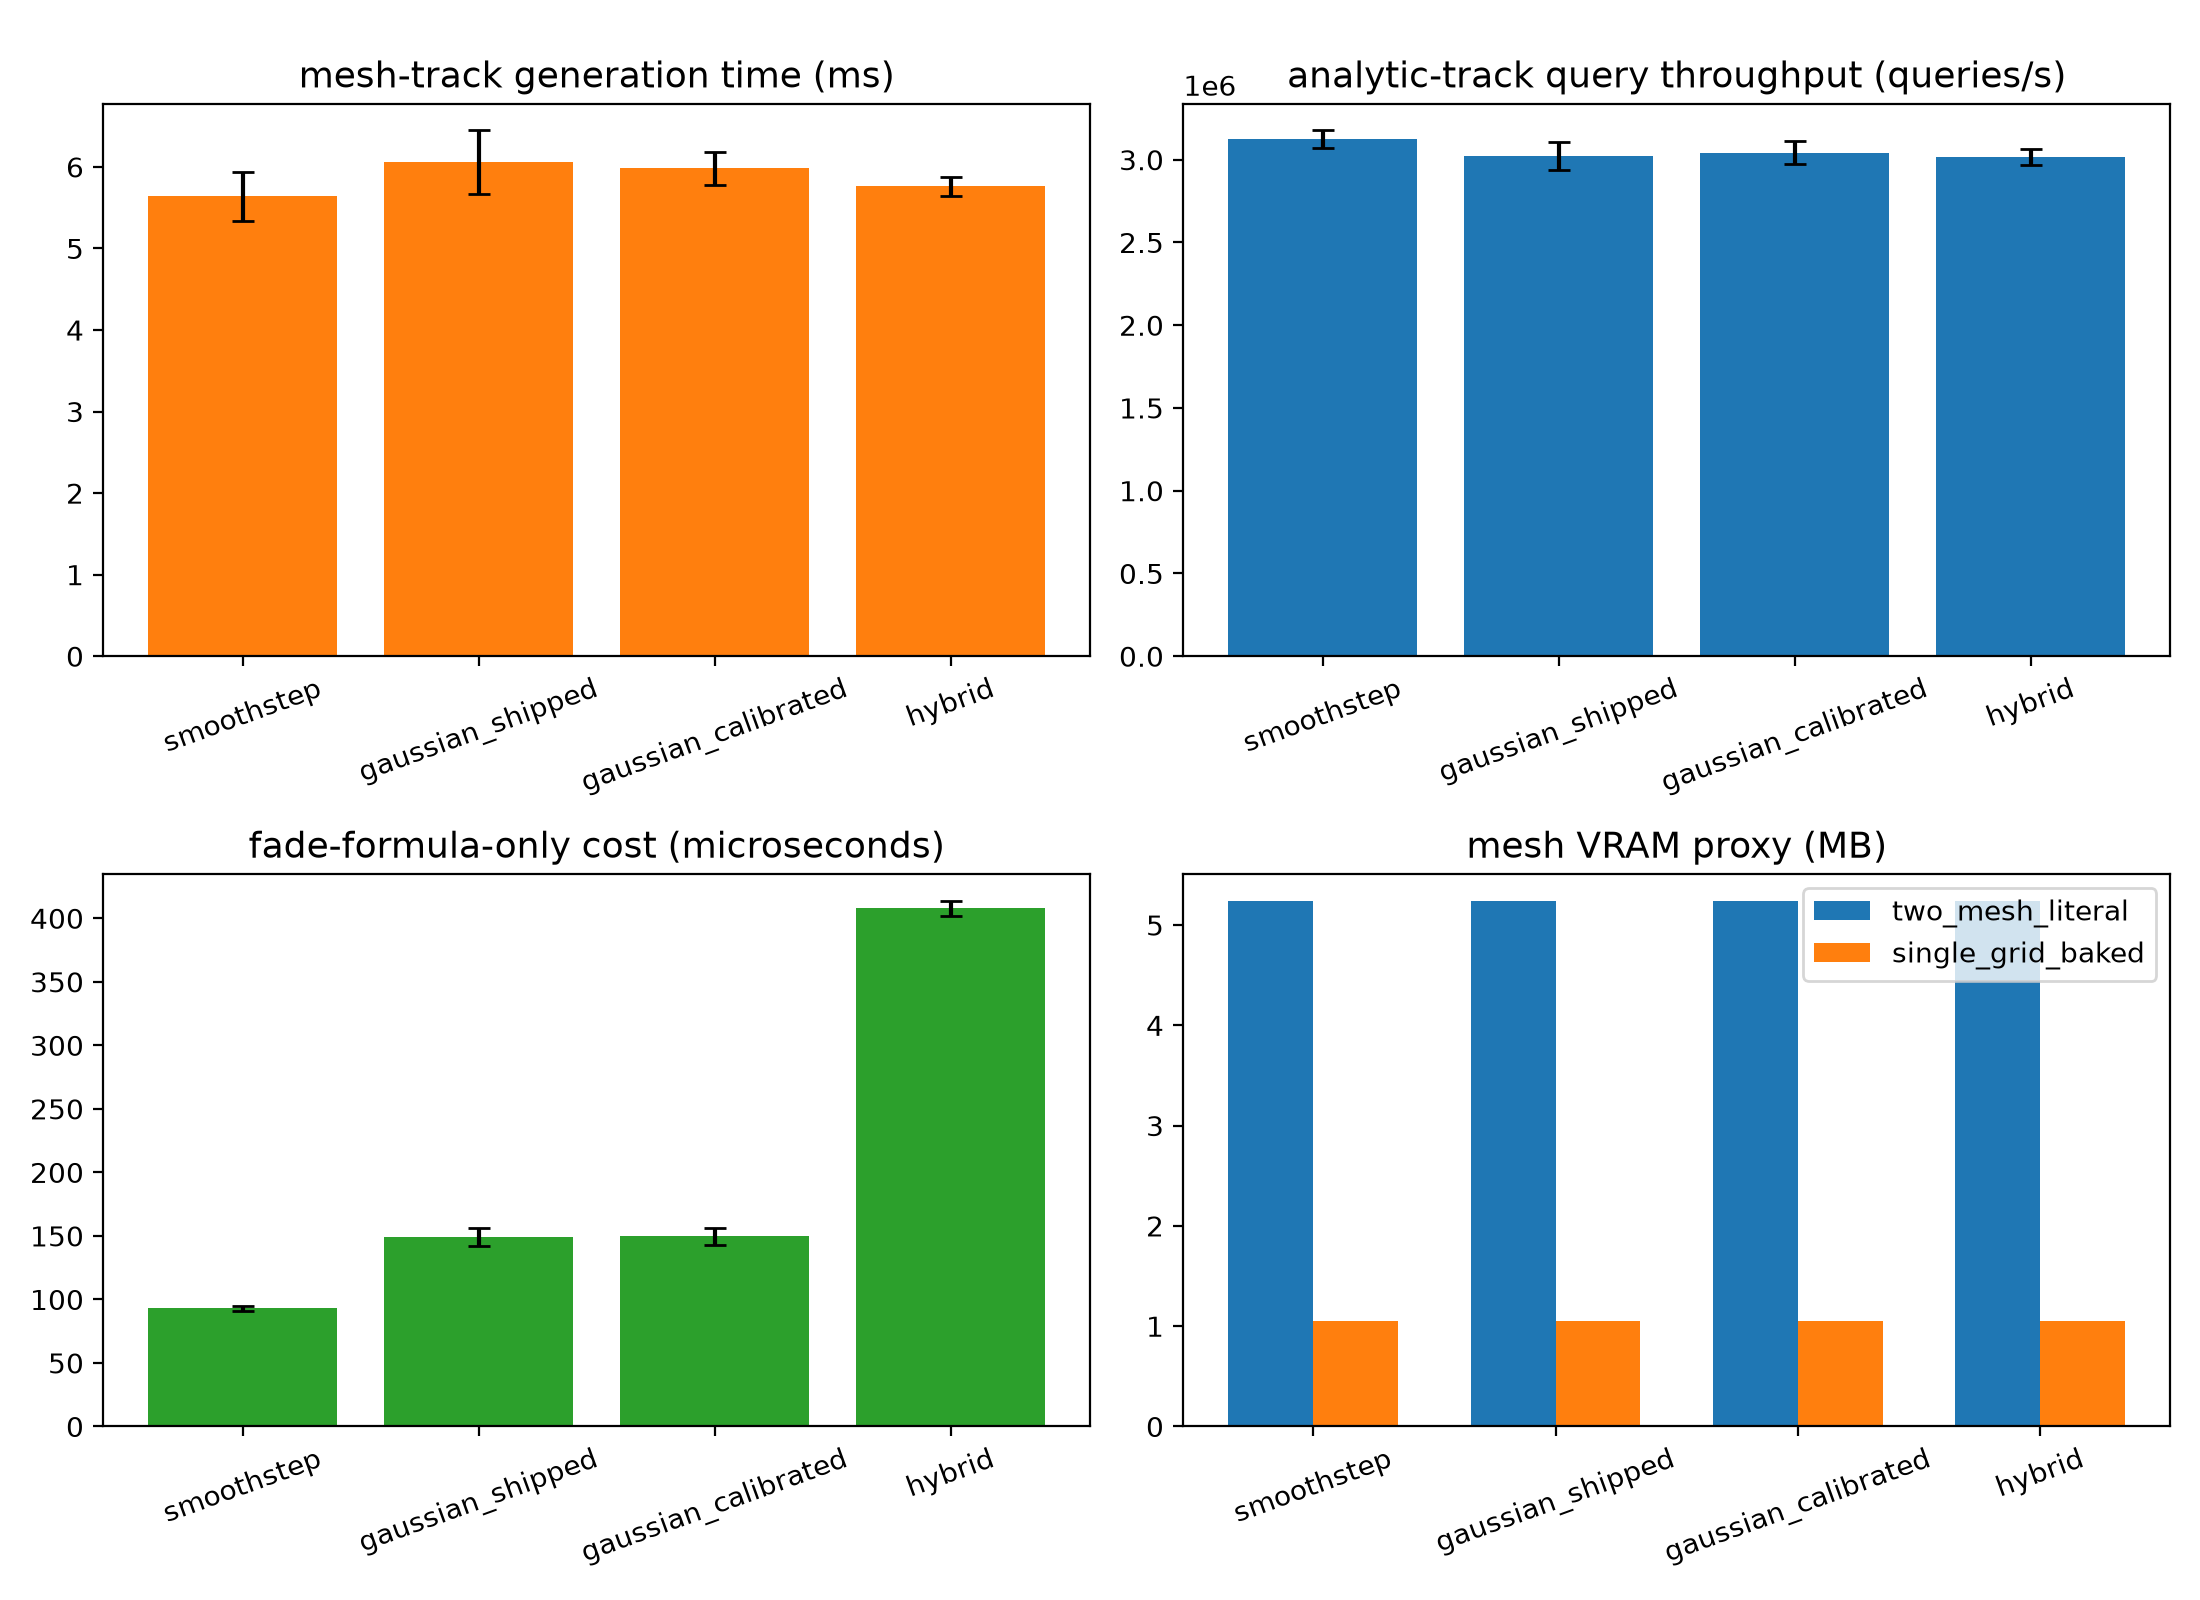
\includegraphics[width=\linewidth]{fig06_cost_comparison.png}
\caption{Yöntemler arası hesaplama maliyeti karşılaştırması.}
\label{fig:cost-comparison}
\end{figure}

\subsection{Ablasyon Analizleri}
\label{sec:ablasyon}

Bu bölüm, önerilen hibrit yöntemin dört tasarım parametresine (temas
yarıçapı, switch genişliği, geçiş yarıçapı, grid çözünürlüğü) karşı
sağlamlığını sınayan dört ayrı ablasyon analizini sunmaktadır.

Hibrit yöntemin temas yarıçapı ($r_c$) taramasında (1,0--4,0~m;
\cref{fig:ablation-rc}), switch'in kendi iç geçiş sınırındaki ($r=r_c$)
C0 süreksizliği tüm $r_c$ değerlerinde $3\times10^{-4}$~m'nin altında
kalmış ve söndürme maliyeti $r_c$'den bağımsız olarak sabit (yaklaşık
755--793 mikrosaniye) kalmıştır; bu, maliyetin switch'in nerede
konumlandığından değil, iki dalın da her durumda hesaplanmasından
kaynaklandığını doğrulamaktadır.

\begin{figure}[t]
\centering
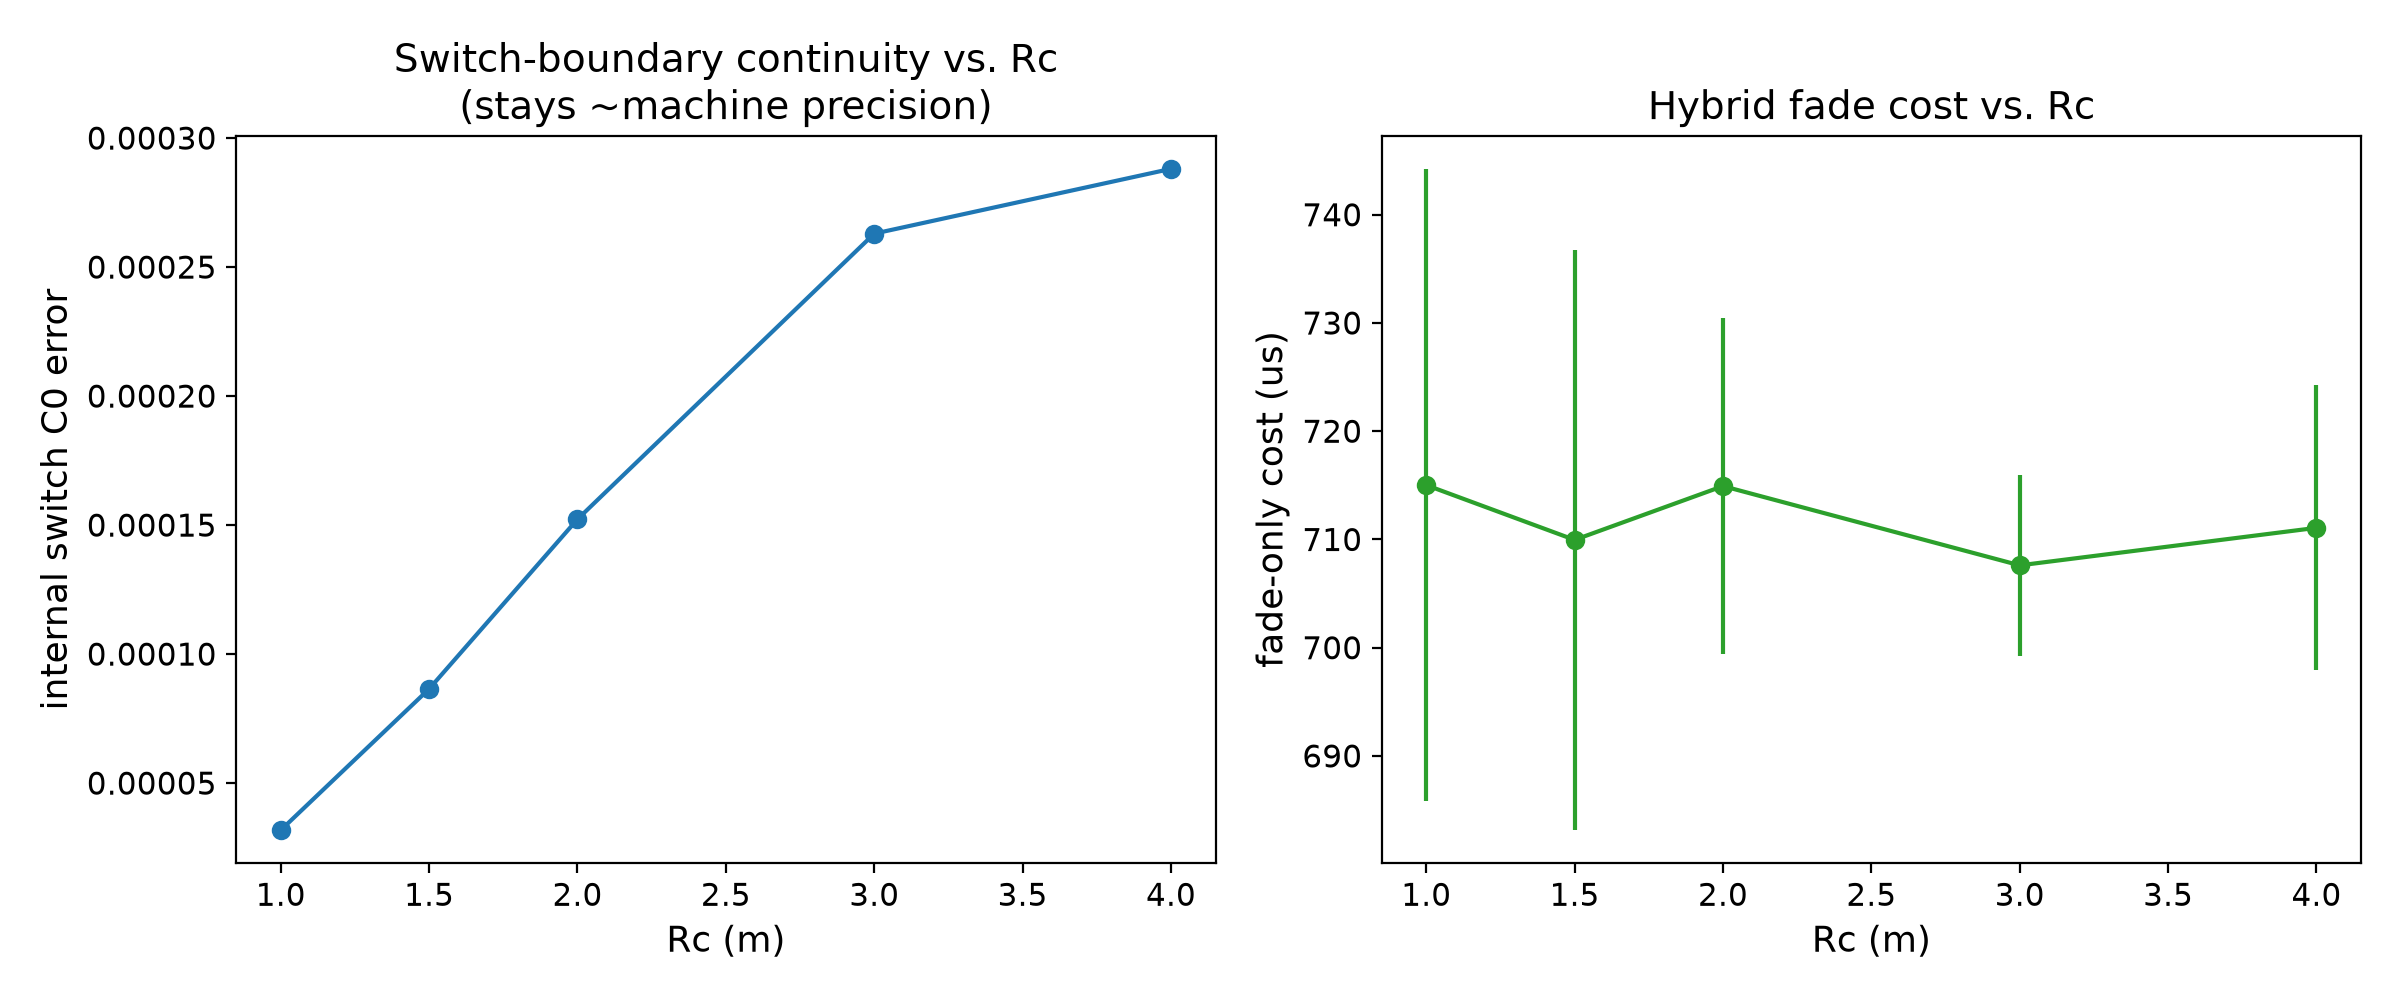
\includegraphics[width=\linewidth]{fig07_ablation_rc.png}
\caption{Temas yarıçapı ($r_c$) taraması: switch iç sürekliliği ve
maliyet.}
\label{fig:ablation-rc}
\end{figure}

Switch genişliği ($w$) taramasında (0,05--2,0~m; \cref{fig:ablation-w}),
switch'in iç sürekliliği $w=0{,}05$~m'de $7{,}03\times10^{-4}$~m'den
$w=1{,}0$~m'de $1{,}74\times10^{-7}$~m'ye kadar düzenli olarak
iyileşmiş, ancak $w=2{,}0$~m'de hafifçe kötüleşmiştir
($1{,}83\times10^{-5}$~m); bu, switch genişliğinin temas yarıçapına yakın
büyüklüklere ulaştığında switch'in yerel eğriliğini bozmaya başladığını
düşündürmekte ve makine hassasiyetine yakın bir iç süreklilik için $w$
yaklaşık 0,3--1,0~m aralığının uygun bir varsayılan olduğunu
göstermektedir; üretim yapılandırmasında kullanılan $w=0{,}3$~m, bu
aralığın içinde bilinçli bir güvenlik marjı sağlamaktadır.

\begin{figure}[t]
\centering
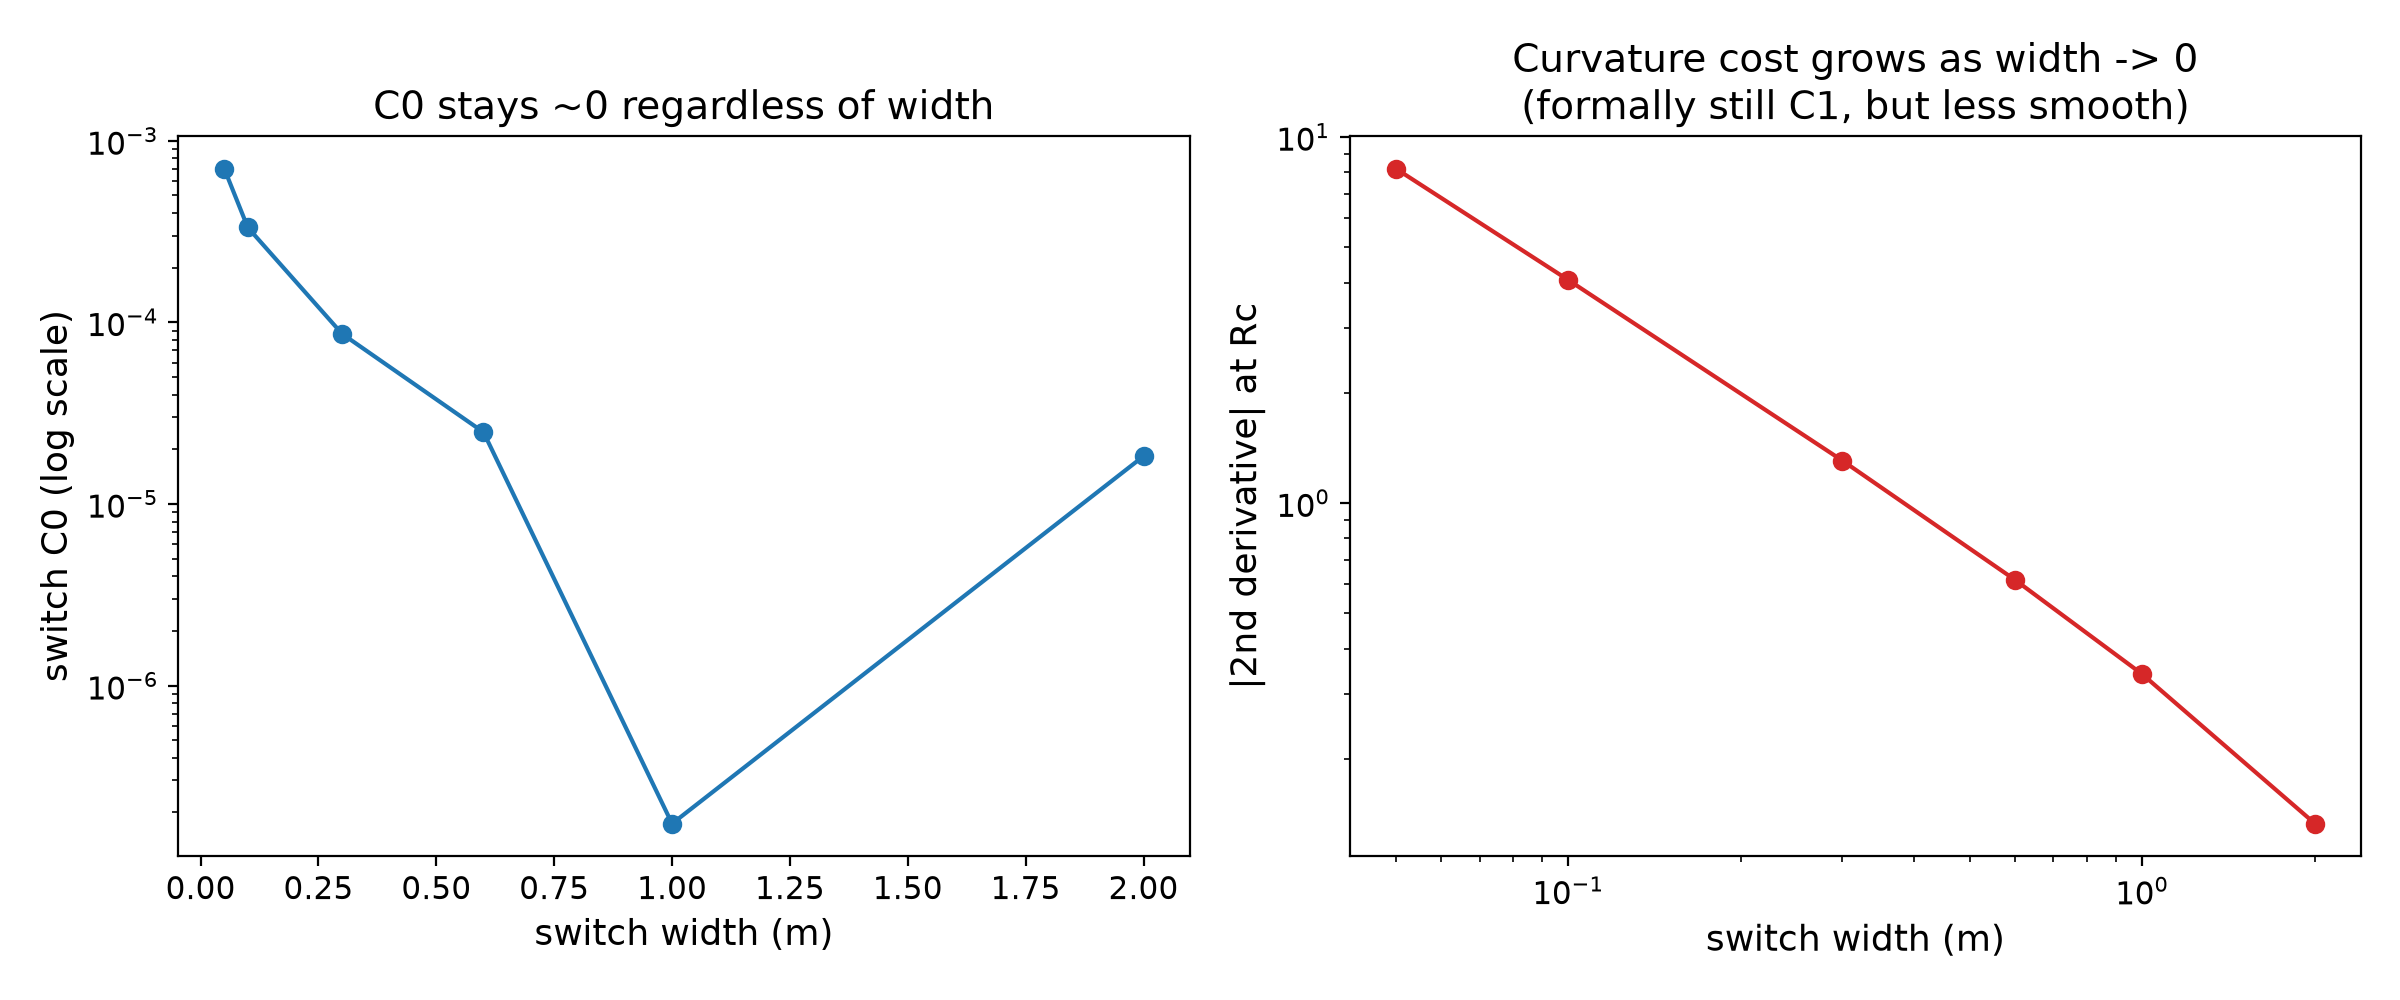
\includegraphics[width=\linewidth]{fig08_ablation_w.png}
\caption{Switch genişliği ($w$) taraması: iç süreklilik.}
\label{fig:ablation-w}
\end{figure}

Bu kusurun geçiş yarıçapından bağımsız olup olmadığını sınamak amacıyla
yapılan yarıçap taramasında ($R=4,6,8,12,16$~m; \cref{fig:ablation-R}),
üretim öncesi Gauss'un C0 (RMS) hatası neredeyse sabit kalmaktadır
(yaklaşık $1{,}68\times10^{-3}$ ile $1{,}76\times10^{-3}$~m arası), yani
hata geçiş yarıçapı büyüdükçe küçülmemektedir; buna karşın smoothstep ve
kalibre edilmiş Gauss'un hatası, yarıçap büyüdükçe (eğrilik azaldıkça)
beklendiği gibi düzenli olarak azalmaktadır. Bu, üretim öncesi Gauss'un
kusurunun bir ayrıklaştırma (discretization) hatası değil, geçiş
yarıçapından bağımsız, ölçek değişmez bir yapısal özellik olduğunu
göstermektedir.

\begin{figure}[t]
\centering
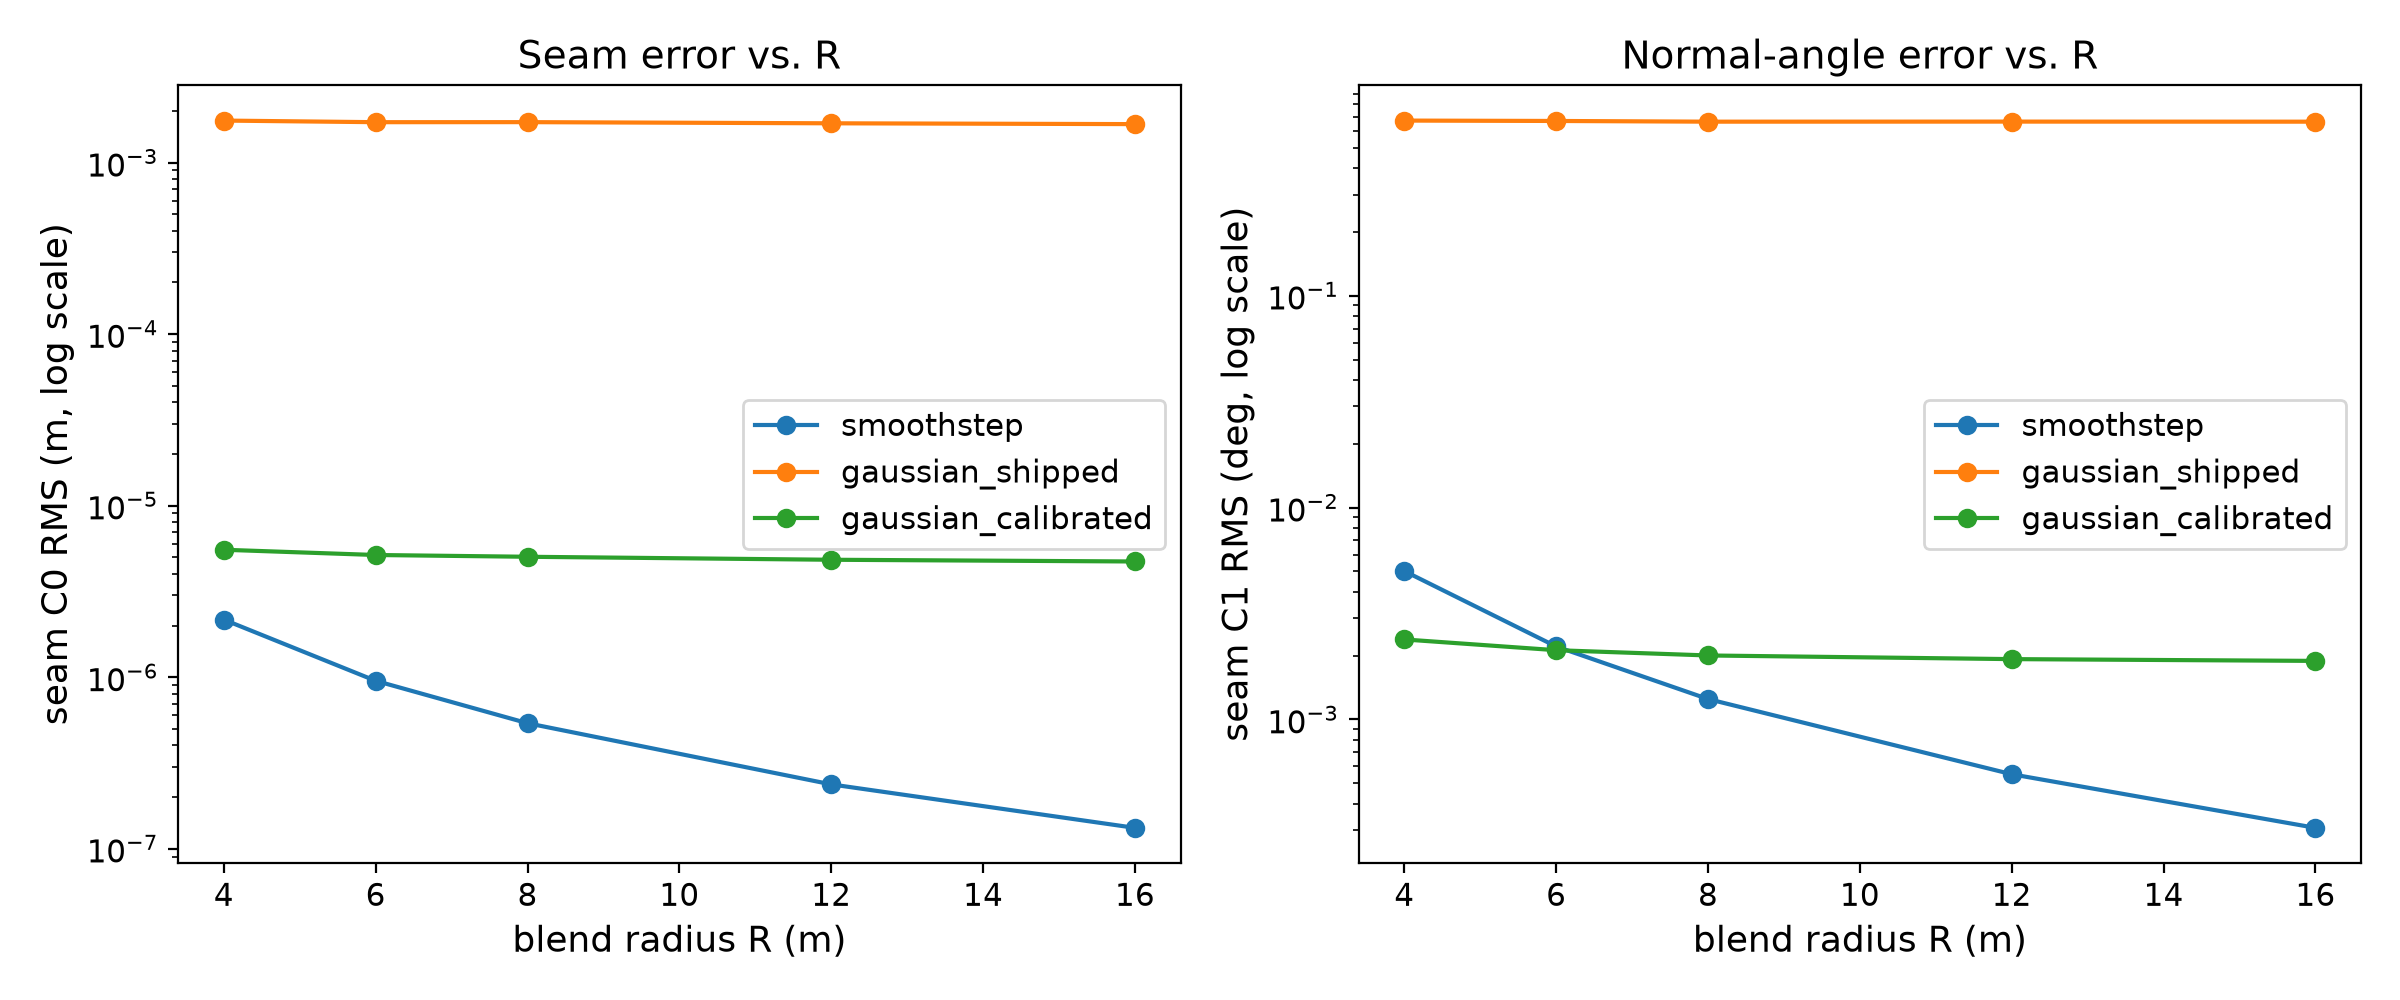
\includegraphics[width=\linewidth]{fig09_ablation_R.png}
\caption{Geçiş yarıçapı ($R$) taraması: ölçek değişmezliği.}
\label{fig:ablation-R}
\end{figure}

Grid çözünürlüğü taramasında (grid aralığı yaklaşık 0,31--1,27~m;
\cref{fig:ablation-grid}), smoothstep ve hibrit yöntemlerin ampirik
yakınsama derecesi (log-log doğrusal regresyon eğimi) yaklaşık 0,90
olarak ölçülmüş, yani hata çözünürlük arttıkça beklenen şekilde
azalmaktadır. Kalibre edilmiş Gauss'ta ise negatif bir eğim (yaklaşık
$-0{,}36$) gözlenmiştir; ancak bu bir fiziksel ``çözünürlük arttıkça
kötüleşme'' bulgusu değildir -kalibre edilmiş Gauss'un hatası zaten
$10^{-6}$ ile $10^{-7}$~m mertebesinde, kalibrasyon sabitinin
belirlediği sabit bir kesme-kalıntısı gürültü tabanına yakındır ve bu
taban, grid çözünürlüğünden bağımsız bir ölçüm sınırı oluşturmaktadır; bu
husus, yanıltıcı bir fiziksel yorumdan kaçınmak için burada açıkça
belirtilmektedir.

\begin{figure}[t]
\centering
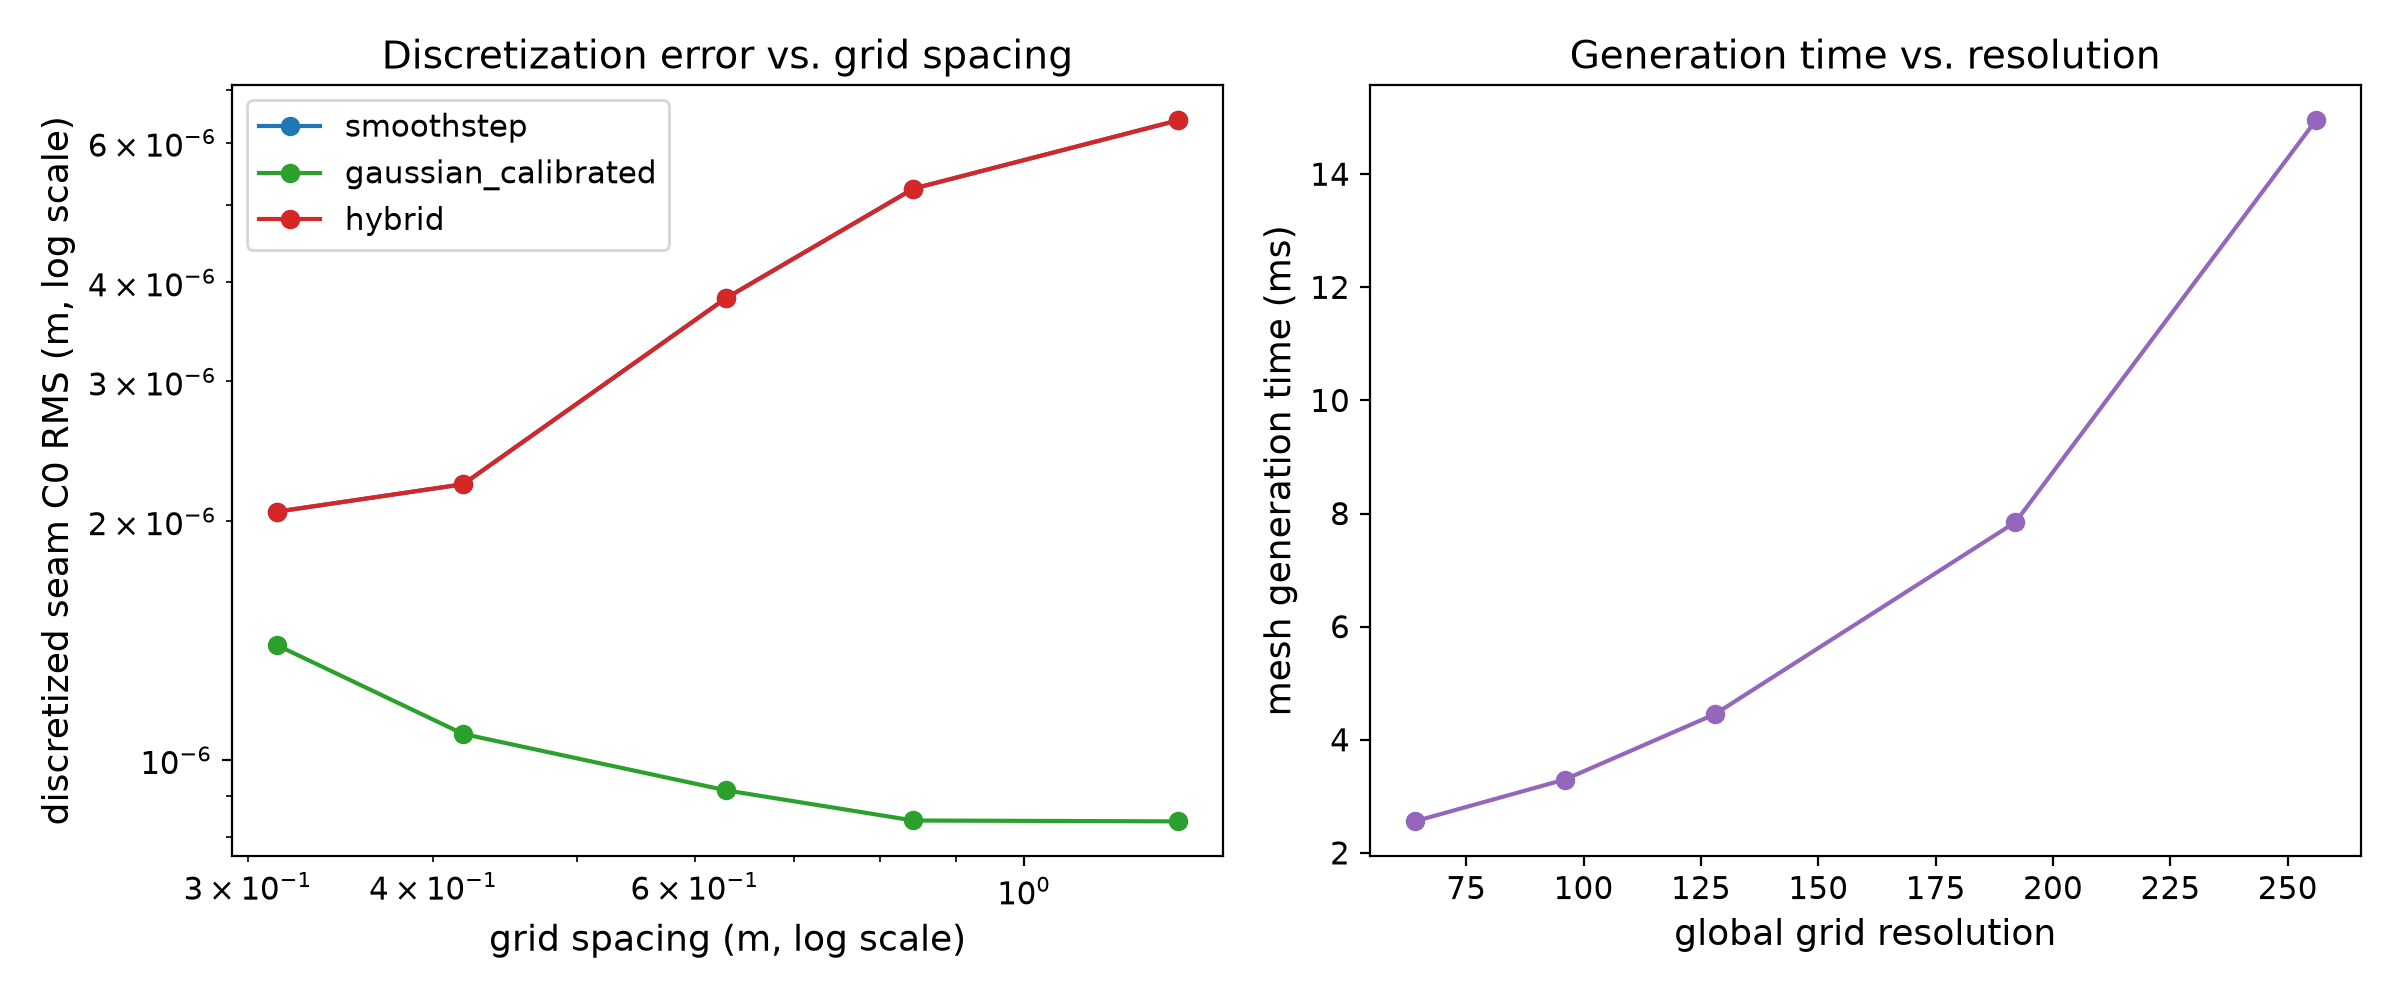
\includegraphics[width=\linewidth]{fig10_ablation_grid.png}
\caption{Grid çözünürlüğü taraması: ampirik yakınsama derecesi.}
\label{fig:ablation-grid}
\end{figure}

Dört analizin ortak sonucu, önerilen hibrit yöntemin süreklilik
avantajının, makul bir parametre aralığında ($r_c=1{,}0$--$4{,}0$~m,
$w=0{,}3$--$1{,}0$~m) sağlam (robust) olduğu, yani belirli bir ince
ayara aşırı duyarlı olmadığıdır. Tek istisna, çok dar switch
genişliklerinde ($w\le 0{,}1$~m) iç sürekliliğin gözle görülür biçimde
bozulmasıdır; bu, üretim yapılandırmasında ($w=0{,}3$~m) kullanılan
varsayılanın bilinçli bir güvenlik marjı içerdiğini bir kez daha
doğrulamaktadır.

\subsection{Gerçek Isaac Sim Eğitim Sonuçları}
\label{sec:egitimsonuclari}

Dokuz eğitim koşusunun (3 yöntem x 3 tohum) tamamı hatasız
tamamlanmış, her biri 5.734.400 ortam adımına ulaşmıştır
(\cref{tab:training}). Duvar saati (wall-clock) süresi, yöntem
ortalaması olarak smoothstep için $2377\pm 98$~s, kalibre edilmiş Gauss
için $2850\pm 898$~s ve hibrit için $2674\pm 599$~s'dir. Bu ortalamalar,
ilk (seed=42) koşularda gözlenen büyük farkın (Gauss ve hibrit sırasıyla
\%56 ve \%35 daha yavaş) çoklu tohumla büyük ölçüde küçüldüğünü
göstermektedir: seed=7 ve seed=123 koşularının üçü de birbirine yakın
(2318--2345~s) sürerken, yalnızca seed=42'deki Gauss ve hibrit koşuları
belirgin biçimde daha yavaştır. Standart sapmaların büyüklüğü (898 ve
599~s, ortalamanın \%20--30'u) bu tek-koşu sapmasının kaynağıdır;
dolayısıyla ilk ölçümdeki ``\%35--56 daha yavaş'' bulgusu, karıştırma
formülünün kendisinden değil, o belirli koşuya özgü sistem-düzeyi bir
değişkenlikten (arka plan yükü, termal durum veya terrain havuzu
zamanlaması) kaynaklanmış olabilir; üç tohumun ortalamasına bakıldığında
Gauss ve hibrit hâlâ smoothstep'ten yavaş görünmektedir (+\%20 ve
+\%12,5) ama bu fark artık ilk ölçümdeki kadar keskin değildir.

\begin{table}[t]
\centering
\caption{Gerçek Isaac Sim eğitiminde son yüzde onluk pencere özeti
(yöntem başına üç tohum).}
\label{tab:training}
\footnotesize
\begin{tabular}{@{}lccccc@{}}
\toprule
\textbf{Method} & \textbf{$n$} & \textbf{Wall time (s)} & \textbf{Success rate} & \textbf{Timeout rate} & \textbf{Harsh-landing} \\
\midrule
smoothstep & 3 & $2377\pm 98$ & $0.278\pm 0.055$ & $0.499\pm 0.059$ & $0.220\pm 0.022$ \\
gaussian (cal.) & 3 & $2850\pm 898$ & $0.325\pm 0.051$ & $0.454\pm 0.074$ & $0.218\pm 0.038$ \\
hybrid & 3 & $2674\pm 599$ & $0.268\pm 0.025$ & $0.515\pm 0.019$ & $0.214\pm 0.007$ \\
\bottomrule
\end{tabular}
\end{table}

Son yüzde on penceresinde ölçülen nihai başarı oranı, yöntem ortalaması
olarak smoothstep için \%27,8~$\pm$~\%5,5, kalibre edilmiş Gauss için
\%32,5~$\pm$~\%5,1 ve hibrit için \%26,8~$\pm$~\%2,5 olarak bulunmuştur
(\cref{tab:training}). Gauss'un ortalaması hâlâ en yüksektir, ancak üç
yöntemin standart sapmaları birbirleriyle örtüşmektedir. \Cref{tab:pairwise},
bu farkların ikili istatistiksel testlerini özetlemektedir: hiçbir ikili
karşılaştırma istatistiksel olarak anlamlı değildir; başarı oranında
smoothstep-Gauss $p=0{,}20$, smoothstep-hibrit $p=1{,}00$, Gauss-hibrit
$p=0{,}40$; zaman aşımı oranında sırasıyla $p=0{,}70$, $p=1{,}00$,
$p=0{,}40$; sert iniş oranında üçü de $p\ge 0{,}70$. Bootstrap \%95 güven
aralıklarının tamamı sıfırı kapsamaktadır (ör.\ Gauss-hibrit başarı
oranı farkı için $[-0{,}000,\,0{,}104]$ -sınırda ama sıfırı içeriyor).

\begin{table}[t]
\centering
\caption{Son yüzde onluk pencere üzerinde ikili karşılaştırmalar
(Mann-Whitney U, betimsel; bkz. \cref{sec:egitimprotokolu} çekincesi).}
\label{tab:pairwise}
\footnotesize
\begin{tabular}{@{}llcccc@{}}
\toprule
\textbf{Metric} & \textbf{Comparison} & \textbf{$n$} & \textbf{Mean diff} & \textbf{95\% CI} & \textbf{MW $p$} \\
\midrule
Success rate & smoothstep vs gaussian & 3 vs 3 & $-0.047$ & $[-0.112, 0.018]$ & 2.00e-01 \\
Success rate & smoothstep vs hybrid & 3 vs 3 & $0.010$ & $[-0.040, 0.068]$ & 1.00e+00 \\
Success rate & gaussian vs hybrid & 3 vs 3 & $0.057$ & $[-0.000, 0.104]$ & 4.00e-01 \\
Timeout rate & smoothstep vs gaussian & 3 vs 3 & $0.045$ & $[-0.044, 0.133]$ & 7.00e-01 \\
Timeout rate & smoothstep vs hybrid & 3 vs 3 & $-0.017$ & $[-0.073, 0.039]$ & 1.00e+00 \\
Timeout rate & gaussian vs hybrid & 3 vs 3 & $-0.061$ & $[-0.132, 0.008]$ & 4.00e-01 \\
Harsh-landing & smoothstep vs gaussian & 3 vs 3 & $0.002$ & $[-0.041, 0.040]$ & 1.00e+00 \\
Harsh-landing & smoothstep vs hybrid & 3 vs 3 & $0.006$ & $[-0.012, 0.031]$ & 1.00e+00 \\
Harsh-landing & gaussian vs hybrid & 3 vs 3 & $0.004$ & $[-0.027, 0.047]$ & 7.00e-01 \\
\bottomrule
\end{tabular}
\end{table}

\Cref{fig:training-curves}, üç yöntemin dokuz koşusunun tamamını üç ana
sonuç metriği (başarı, zaman aşımı, sert iniş oranı) için aynı grafik
üzerinde göstermektedir; dokuz eğrinin de eğitim boyunca büyük ölçüde iç
içe geçmiş olması, yöntemler arası farkın tohumlar arası varyanstan
görsel olarak ayırt edilemediğini doğrulamaktadır. \Cref{fig:training-diag},
aynı dokuz koşu için müfredat zorluğu, entropi katsayısı ve
xy-ilerleme ödülü gibi tamamlayıcı eğitim diyagnostiklerini
göstermektedir; entropi katsayısının üç yöntemde de neredeyse özdeş bir
yakınsama eğrisi izlemesi, SAC'ın keşif-sömürü dengesinin karıştırma
yöntemi seçiminden bağımsız işlediğine işaret etmektedir.
\Cref{fig:final-window-box}, son yüzde onluk pencere değerlerini yöntem
başına dağılım noktaları ve ortalama $\pm$ standart sapma çubuğu olarak
sunmaktadır; üç yöntemin hata çubuklarının geniş ölçüde örtüştüğü buradan
da açıkça görülmektedir.

\begin{figure}[t]
\centering
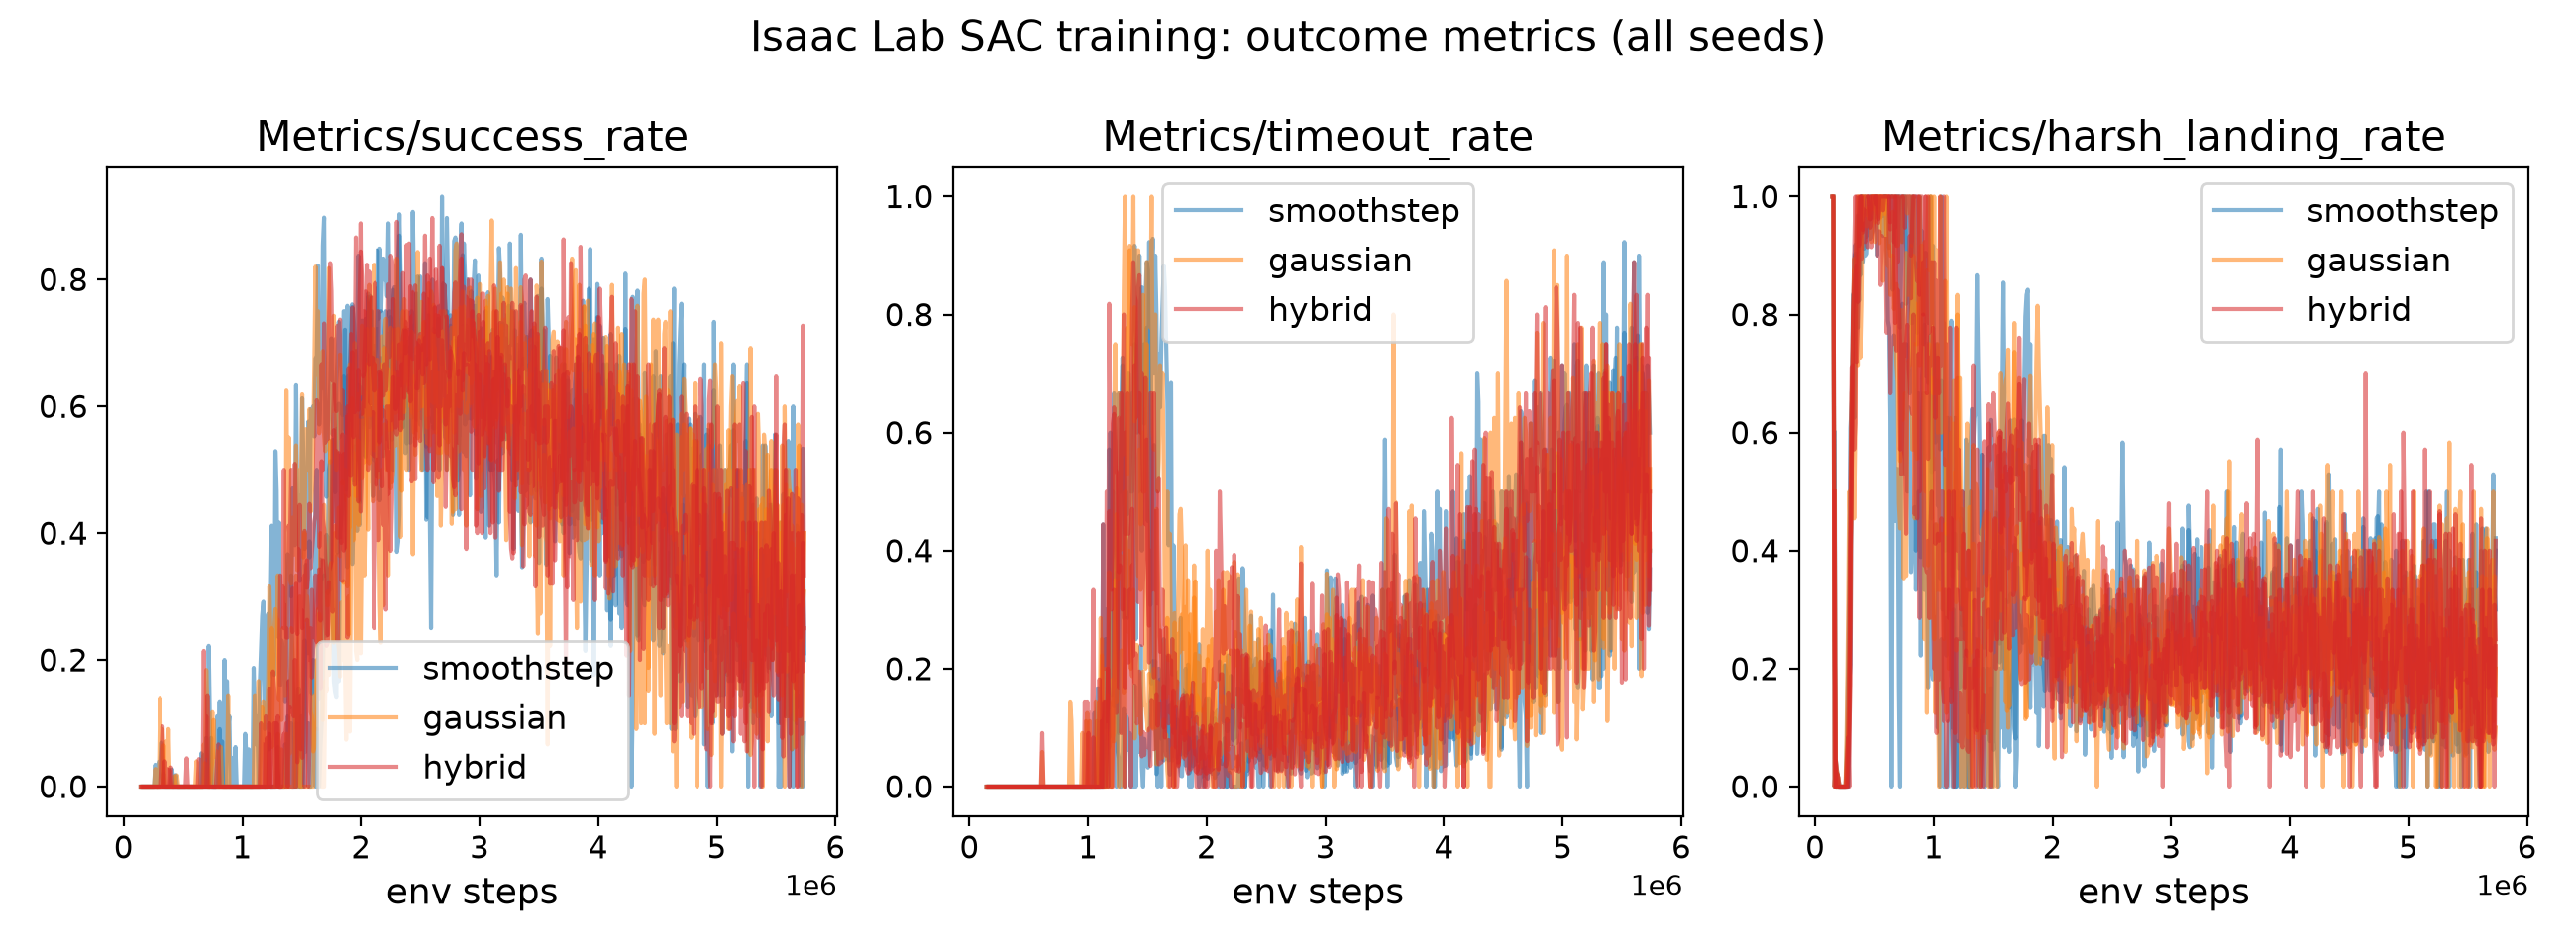
\includegraphics[width=\linewidth]{fig11_training_curves.png}
\caption{Üç yöntem için eğitim boyunca izlenen sonuç metrikleri
(başarı/zaman aşımı/sert iniş oranı).}
\label{fig:training-curves}
\end{figure}

\begin{figure}[t]
\centering
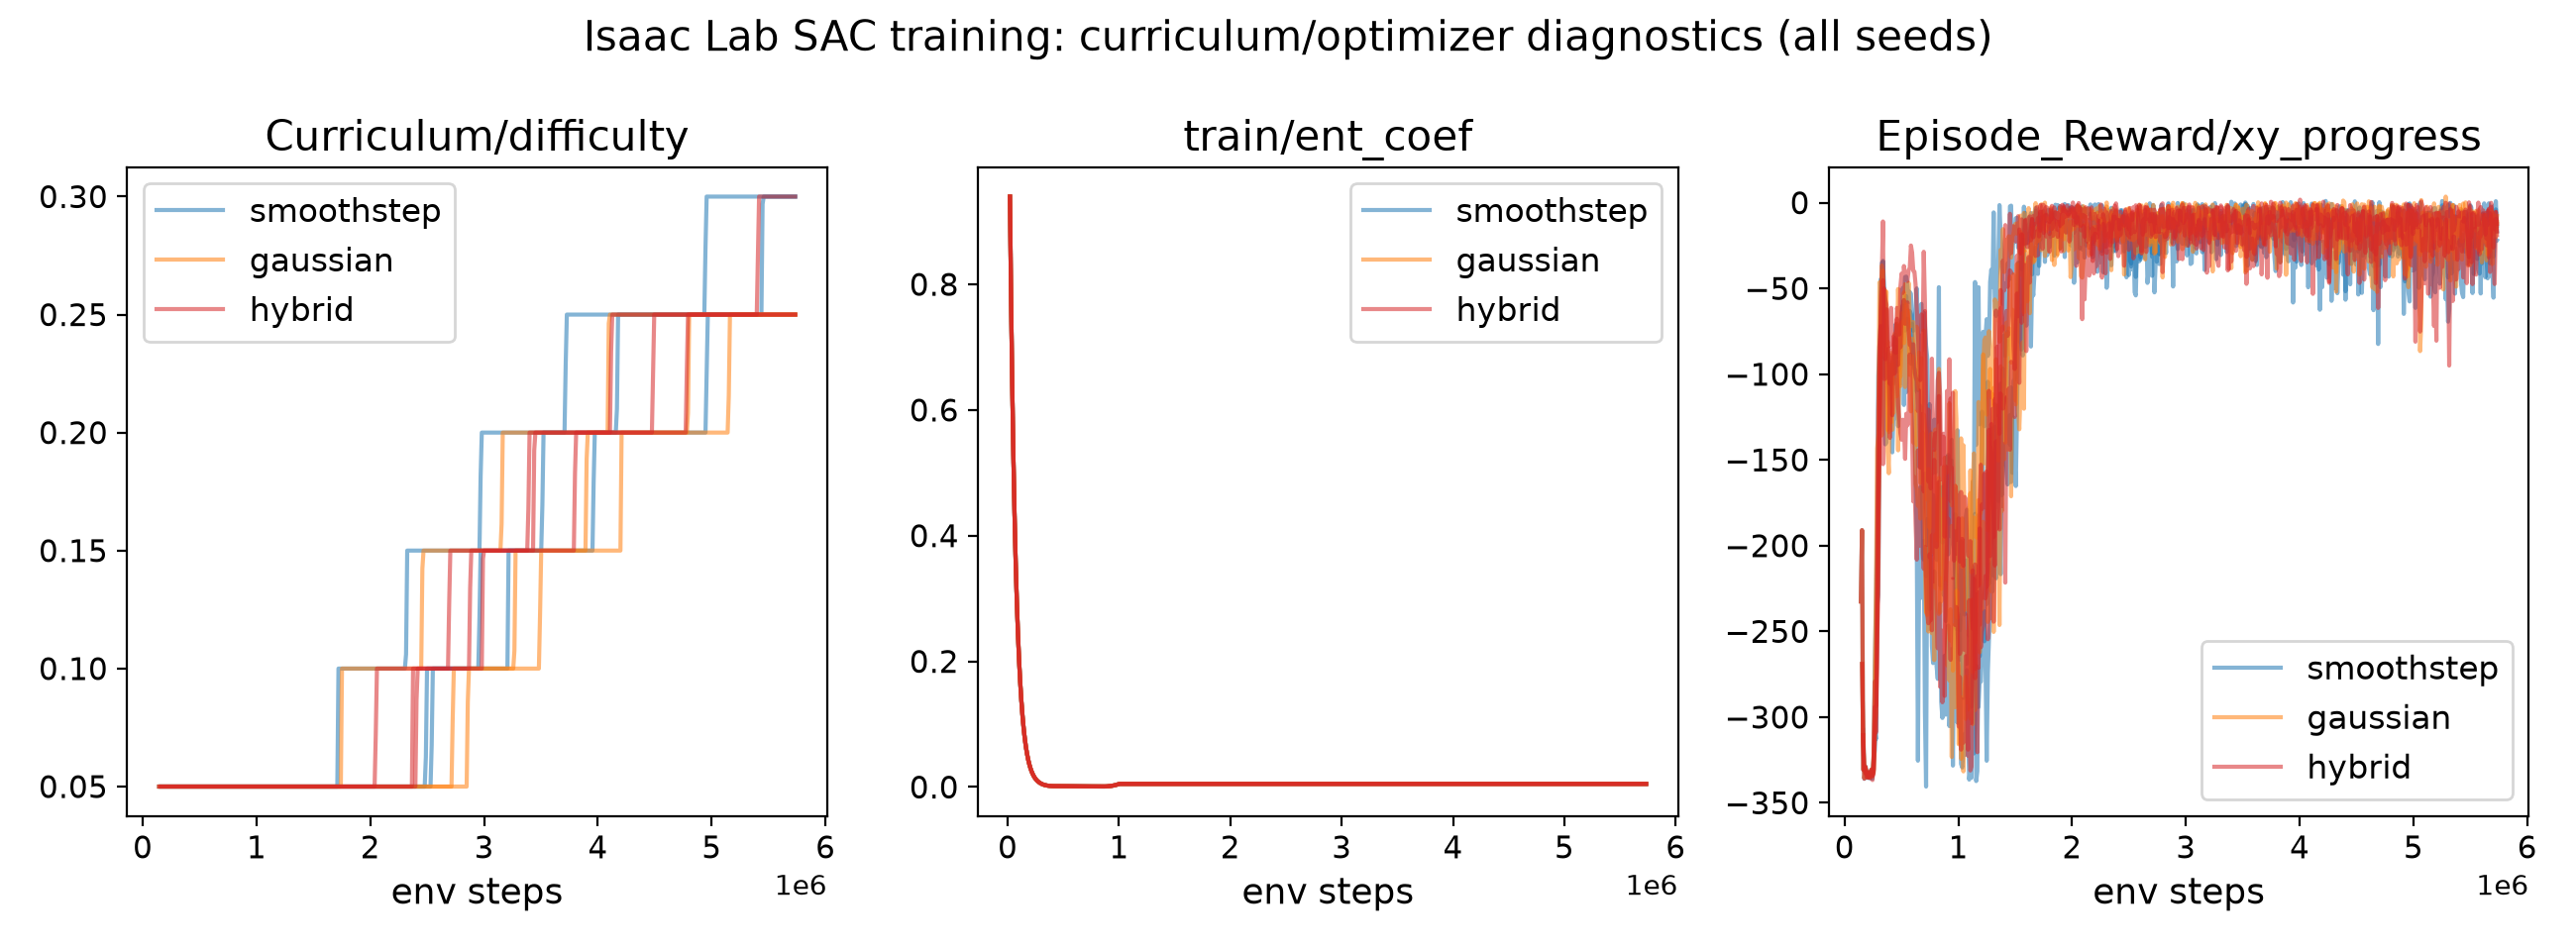
\includegraphics[width=\linewidth]{fig12_training_diagnostics.png}
\caption{Üç yöntem için eğitim boyunca izlenen tamamlayıcı
diyagnostikler (müfredat zorluğu, entropi katsayısı, xy-ilerleme ödülü).}
\label{fig:training-diag}
\end{figure}

\begin{figure}[t]
\centering
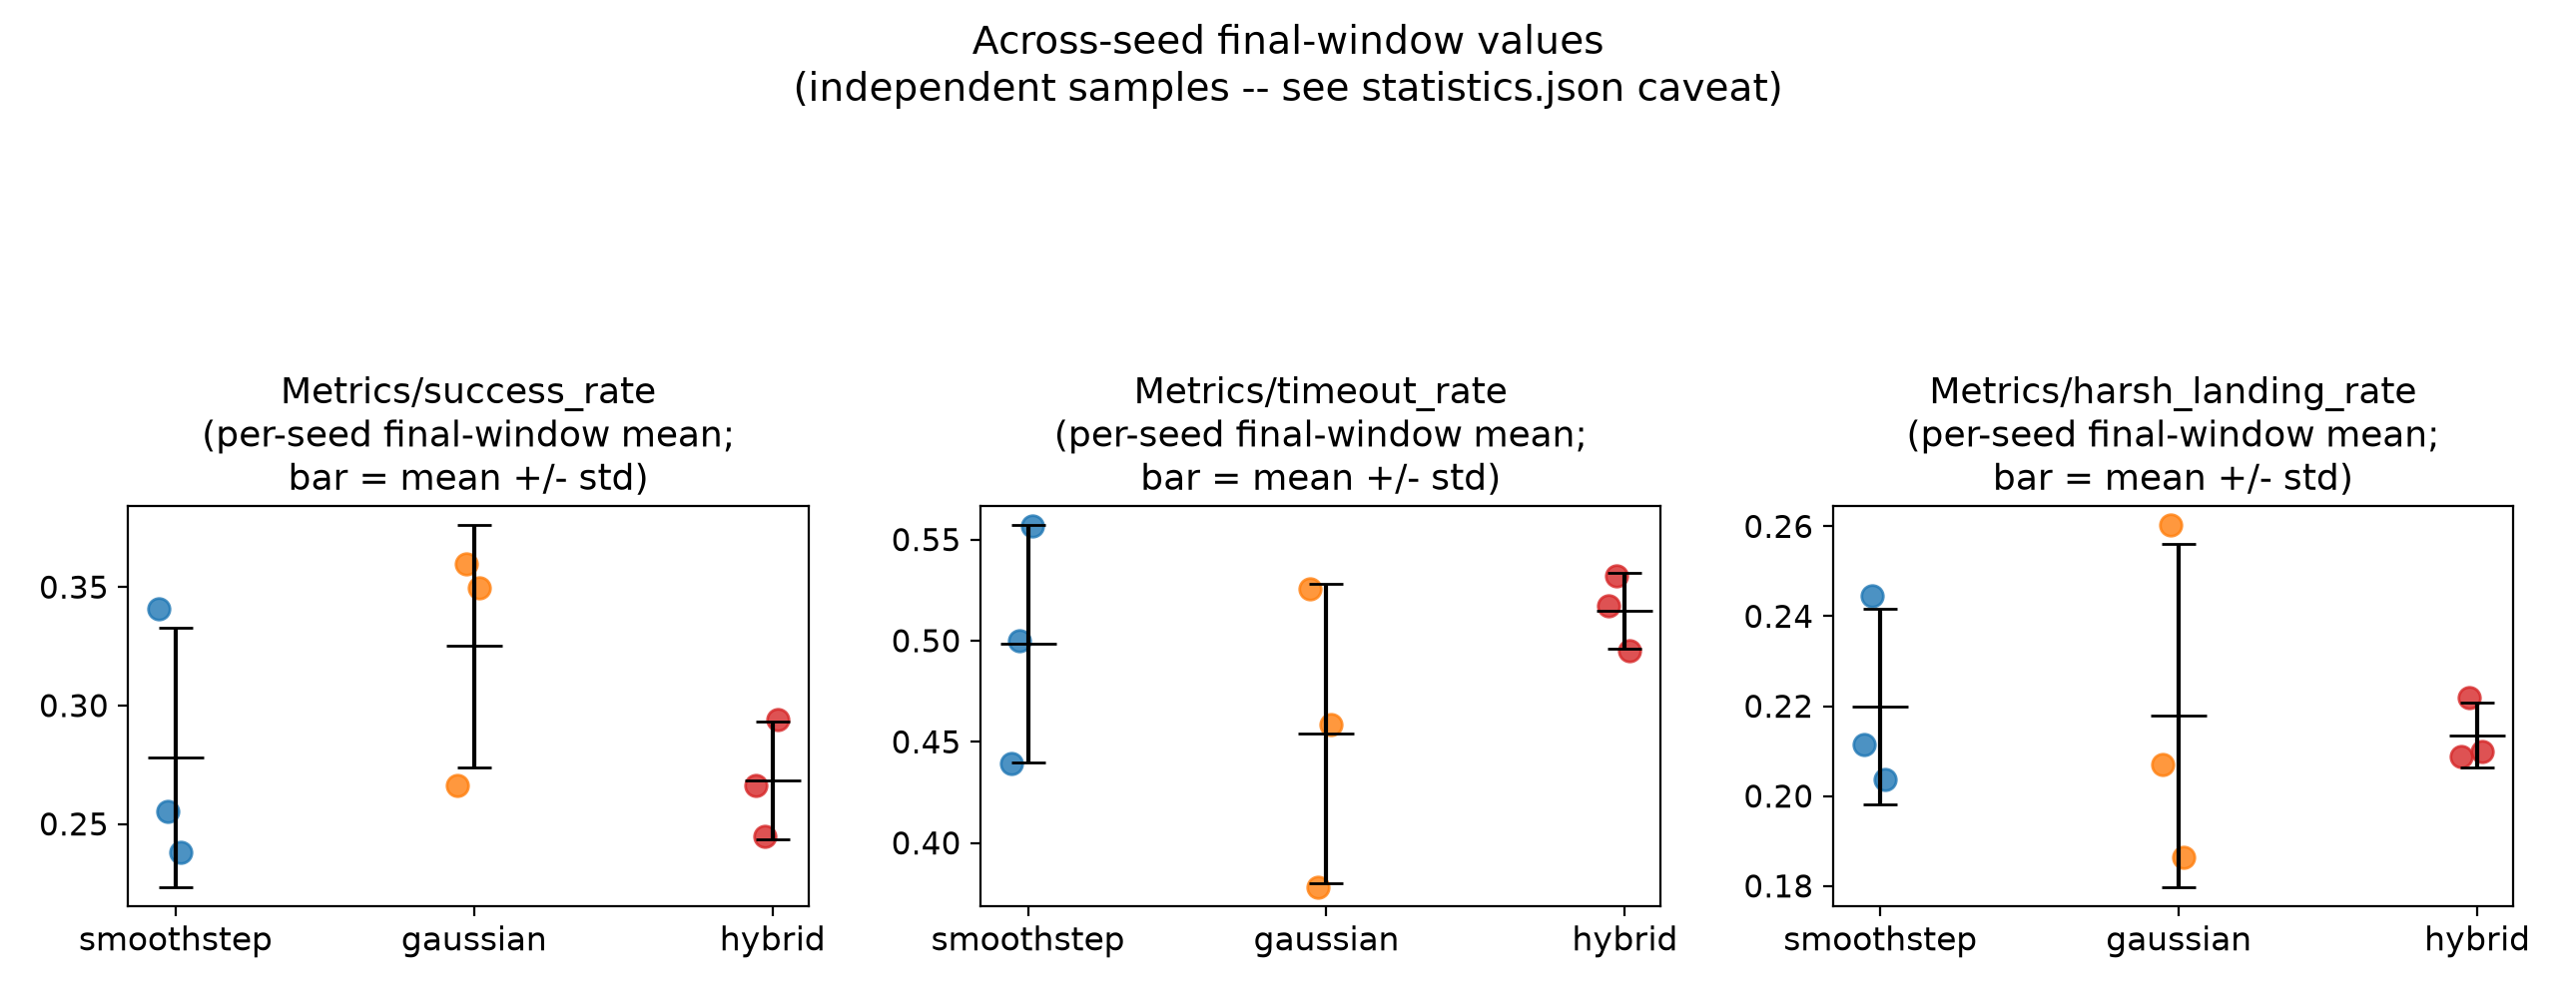
\includegraphics[width=\linewidth]{fig13_final_window_box.png}
\caption{Son yüzde onluk pencere dağılımları (kutu grafiği).}
\label{fig:final-window-box}
\end{figure}

Bu sonuç, ilk (tek tohumlu) ölçümde gözlenen ve \cref{sec:tartisma}'te
ayrıntılı olarak tartışılan ``Gauss ve hibrit'in smoothstep'ten anlamlı
derecede daha başarılı olduğu'' bulgusunu doğrulamamaktadır. $n=1$'den
$n=3$'e çıkıldığında etki büyüklüğü küçülmüş (Gauss-smoothstep farkı
\%11'den \%4,7'ye düşmüş) ve yön kısmen değişmiştir
(hibrit-smoothstep farkı işaret değiştirmiştir: ilk ölçümde hibrit
smoothstep'ten yüksekti, üç-tohum ortalamasında hibrit smoothstep'e
neredeyse eşittir, hatta hafifçe düşüktür). Bu örüntü, ilk bulgunun -en
azından büyük ölçüde- rastgele koşu-koşu varyansıyla tutarlı olduğunu
göstermektedir; bu husus \cref{sec:tartisma}'te ayrıntılı olarak
tartışılmaktadır.

Sample-efficiency ölçütlerinde de benzer bir görünüm vardır: AUC (eğitim
boyunca ortalama başarı oranı) yöntem başına üç tohum arasında geniş bir
aralıkta değişmektedir (smoothstep 0,381--0,395, Gauss 0,366--0,402,
hibrid 0,339--0,399) ve yöntemler arası fark, tohumlar arası farktan
belirgin biçimde küçüktür -bu da yine tohum varyansının baskın kaynak
olduğuna işaret etmektedir.

Müfredat zorluğu, üç yöntemde de ortalama olarak birbirine yakındır
(smoothstep $0{,}276\pm 0{,}025$, Gauss $0{,}250\pm 0{,}000$, hibrit
$0{,}260\pm 0{,}017$); Gauss'un üç tohumda da tam olarak $0{,}25$'te
sabit kalması (sıfır standart sapma) dikkat çekicidir ve rolling-window
başarı eşiğinin bu üç koşuda da aynı basamakta durduğunu göstermektedir
-bu, ilk ölçümde öne sürülen ``Gauss'un yüksek ortalama başarıya rağmen
müfredatta geride kaldığı'' gözlemiyle tutarlıdır, ancak nedeni doğrudan
test edilmemiştir.

\section{Discussion}
\label{sec:tartisma}

The findings first give a clear answer to RQ1: the seam left by the
as-shipped Gaussian blend when truncated at a finite radius is not a
cosmetic or negligible defect but a structural one, measurable at three
orders of magnitude relative to smoothstep (approximately 3200x in C0,
530x in C1) and statistically highly significant. The source of this
defect is not a coding error but a property of radial basis functions
that has been known for more than fifty years: the Gaussian-type radial
functions defined by Hardy \citep{hardy1971multiquadric} are
infinite-support and never reach exactly zero at any finite radius;
Wendland \citep{wendland1995piecewise} proposed compact-support,
minimal-degree positive-definite radial functions as exactly the
solution to this problem. This study's contribution is to demonstrate
this fifty-year-old mathematical fact quantitatively in a concrete
engineering setting (a physically queryable lunar-terrain height field)
and to test whether it is reflected in RL training. Unlike the RL
results discussed below, this analytic finding is validated over 30
seeds and is not subject to single-run uncertainty; it is therefore the
study's most robust and least debatable finding.

In answer to RQ2, the proposed hybrid method preserves the Gaussian's
soft ``bell'' profile in the contact region and smoothstep's compact
support beyond it, while creating no new seam at its own internal
transition (switch); this is an expected result, consistent with the
partition-of-unity framework described by Ohtake et al.\
\citep{ohtake2003multiscale}: a convex combination of two C1-smooth
functions with a C1-smooth weight is itself C1-smooth. The cost of this
advantage is an approximately 4.3x higher microsecond cost than
smoothstep in computing the pure fade formula (because both branches
must be evaluated). This formula-level cost is reflected only partially
and inconsistently in the real training's wall-clock time: in the
initial (seed=42) measurement, Gaussian and hybrid were 56\% and 35\%
slower, respectively, but averaged over three seeds this gap drops to
20\% and 12.5\%, and the standard deviation (20--30\% of the mean) shows
how much a single run can deviate (\cref{sec:egitimsonuclari}). This
suggests that the real wall-clock difference stems largely from
run-to-run system variability (background load, thermal state, terrain
pool timing), with the pure formula cost contributing only a small and
consistent part; this is a separate observation, not to be
over-interpreted, but one that shows single-run measurements can also be
misleading for cost comparisons.

The answer to RQ3 changed substantially after multiple seeds, and this
change is itself one of the study's most instructive findings. In the
initial (single-seed, seed=42) measurement, Gaussian and hybrid appeared
to reach a final success rate approximately 8--12 percentage points
higher than smoothstep, and this initial draft attributed it to a
mechanism such as ``a difference in the transition-band weight
profile.'' In the measurement extended with two additional independent
seeds (seed=7, seed=123) (\cref{sec:egitimsonuclari}), the cross-method
gap shrank (the Gaussian-smoothstep gap dropped from 11\% to 4.7\%), the
hybrid-smoothstep gap changed sign, and no pairwise comparison was
statistically significant on any of the three metrics (success rate,
timeout rate, harsh-landing rate; all $p\ge 0.20$). Recalling that the
Gaussian variant used in the real training (calibrated, $k=\ln(1000)$)
already has analytic boundary continuity nearly equal to smoothstep's
(\cref{tab:continuity}), this result is in fact an expected consistency:
if there is no measurable difference in boundary continuity, it is not
surprising that there is also no strong difference in RL training
performance. The apparent gap in the initial measurement was most likely
ordinary run-to-run variance stemming from the GPU-parallel PhysX
simulation's own internal nondeterminism and the timing-dependence of
the terrain pool's background CPU generation process --- exactly the
pseudoreplication pitfall warned against by Henderson et al.\
\citep{henderson2018deep}. Because this study thereby refutes its own
initial finding, it offers a self-contained case study on how misleading
single-run RL comparisons can be: going from $n=1$ to $n=3$ was enough to
render an apparently ``significant'' finding statistically
indistinguishable. That said, $n=3$ is still low-powered, and the
present data cannot rule out the presence of a small real effect
(especially given that the Gaussian consistently has the highest
average); a larger number of seeds is needed to reach a definitive
conclusion (\cref{sec:sonuc}).

The scope of this study was deliberately kept narrow in order to isolate
the effect of the blending function as a single variable; the three
methods were compared only against each other, with the rest of the
production environment (physics engine, reward function, agent
architecture, curriculum schedule) held fixed. Bringing in another
terrain-blending method from the literature --- e.g., one implemented in
a different simulator --- as an external benchmark was deliberately not
chosen; such a comparison would make it impossible to separate the
effect of the blending function from the countless other differences in
that simulator's physics engine, observation/reward design, and agent
architecture. The cost of this choice is that the extent to which the
findings generalize beyond this specific environment (Isaac Lab/PhysX,
SAC, this task definition) --- external validity --- was not tested in
this study; this point is addressed as a concrete future-work direction
in \cref{sec:sonuc}.

The most important limitation of this study is that, with $n=3$, it
still has low statistical power: the smallest $p$-value the Mann-Whitney
test can produce is already bounded with the current data (around a
minimum of $p\approx 0.10$ for a 3-vs-3 comparison), so an ``no
significant difference'' finding does not prove that the methods are
truly equivalent --- it only shows that the seemingly large gap in the
initial measurement could not be reliably confirmed. The second
limitation is that the training scale (5.73 million steps, approximately
350 iterations) remained below the full-scale configuration (1200
iterations) owing to the computational budget; no run may have reached
full convergence, meaning the observed plateaus may reflect an
interim-stage performance difference rather than a final/asymptotic one.
The third limitation is that the analytic/CPU study isolates only the
fade formula itself and does not fully disentangle the source of the
real-training wall-clock difference (terrain generation, physics
stepping, system variability) --- the three-seed data show that this gap
shrinks, but do not conclusively identify its source.

\section{Conclusion}
\label{sec:sonuc}

This study systematically examined the shape of the blending function
used where a coarse-resolution global terrain meets a fine-detail local
patch in an Isaac Lab-based lunar-landing environment, both at the
analytic/CPU level and in a real Isaac Sim SAC training run. Analytic
measurements over thirty seeds statistically confirmed that the
previously used as-shipped Gaussian blend produces, once truncated at a
finite radius, boundary continuity worse than smoothstep by three
orders of magnitude, and that this defect is a scale-invariant,
structural property. The proposed hybrid method and a calibrated
Gaussian variant remove this defect to near-machine precision --- this
is the study's most robust and least debatable finding.

The real Isaac Sim training comparison began with a single seed per
method, and the initial measurement showed Gaussian and hybrid reaching
a markedly higher success rate than smoothstep. To test the reliability
of this finding, the study was extended with two additional independent
seeds (total $n=3$), and no statistically significant difference was
found between the methods on any metric. This is the study's second
major contribution: it provides a concrete, self-contained example of
how misleading single-run RL comparisons can be, and empirically
confirms the warning of Henderson et al.\ \citep{henderson2018deep} in
this specific setting. Taken together with the analytic results, this
shows that the choice of blending function has a measurable and robust
effect on boundary continuity, but that this effect --- at least at the
present scale and with $n=3$ --- is not reflected in final RL training
performance in a distinguishable way.

The core contribution of this study is a methodology that tests the
choice of blending function quantitatively, both analytically and at the
level of RL training, in a real Isaac Sim/Isaac Lab environment, rather
than treating it as a purely visual/rendering preference; this
methodology is able to reliably report a ``no significant difference''
result just as well as a positive one. All three methods are integrated
into the production code as a backward-compatible, selectable
configuration, making these findings directly actionable: with the
current data, there is no statistical justification for choosing among
the three methods on RL training performance; the choice can instead be
based on other criteria such as boundary continuity (analytically in
favor of Gaussian and hybrid) or computational cost (in favor of
smoothstep).

\subsection*{Implications for autonomous control system design}
For engineers designing the training pipeline of an autonomous control
system, the key takeaway is not which blending function to prefer but
that a simulator's internal geometry-generation choices are themselves
part of the control system's design space and warrant the same
quantitative scrutiny as the controller or the reward function. A
world-model artifact with a large, statistically confirmed effect on
boundary continuity (here, close to three orders of magnitude) need not
automatically threaten the learned controller's deployed behavior; this
study shows a case where a robust simulation-fidelity defect and a
distinguishable control-performance regression can, at a given training
scale, come apart. The practical implication is that such simulator
artifacts should be audited and corrected on their own engineering
merits --- because a discontinuity in a physically queryable contact
geometry is exactly the kind of defect a real vehicle's contact sensors
would not tolerate --- rather than assumed safe merely because a single
training run did not reveal a resulting control-performance gap.

Three concrete directions are proposed for future work. First, because
$n=3$ still has low statistical power, the real-training comparison
should be extended with at least five to ten more independent seeds to
determine conclusively whether the small observed average differences
(particularly the Gaussian's consistently highest average) reflect a
real effect or residual noise. Second, the training scale should be
extended to the full configuration (1200 iterations) to confirm whether
the observed plateaus reflect an interim-stage rather than a
final/asymptotic performance difference. Third, going beyond the scope
that this study deliberately kept narrow (see \cref{sec:tartisma}), the
external validity of the findings should be tested: repeating the same
three blending methods on a different physics engine, a different
reward/observation design, or a different contact-rich task (e.g.,
quadrupedal locomotion, humanoid standing) would disentangle whether the
findings here depend on the blending function or on other design choices
specific to this particular environment.


\section*{Acknowledgment}
This work was carried out without any external funding or institutional
support, using the author's own computational resources (a local NVIDIA
GPU workstation). The author thanks the NVIDIA team for developing Isaac
Lab and Isaac Sim as open-source software, and the open-source software
libraries used in the experimental infrastructure (Stable-Baselines3,
PyTorch, NumPy, SciPy, TensorBoard).

\section*{Declaration of competing interest}
The author declares that he has no known competing financial interests
or personal relationships related to this work.

\section*{Data and code availability}
The analytic evaluation code used in this study (the NumPy port of the
three blending functions, the continuity/cost metrics, and the ablation
scripts), the production environment code (the Isaac Lab task definition
and the selectable integration of the three methods via
ISAACLAB\_TERRAIN\_BLEND\_METHOD), and the raw experimental outputs (the
thirty-seed continuity measurements, the four ablation sweeps, and the
real-training TensorBoard logs) are stored in the author's project
repository and are available from the author upon reasonable request.
The code is planned to be moved to a publicly accessible repository
during the manuscript review process.

\printcredits

\bibliographystyle{elsarticle-num}
\bibliography{refs}

\bio{photo-haktan}
Haktan Yusuf Güloğlu graduated at the top of his class from Profilo
Vocational and Technical Anatolian High School and is currently an
undergraduate student in Computer Engineering at Sakarya University. He
works as a student researcher at Sakarya University's National
Technology Workshop Artificial Intelligence Center, where his research
interests center on reinforcement learning, procedural simulation
environments, and the numerical accuracy of contact geometry in physics
engines. He carried out this study's entire pipeline --- from
conceptualization and experimental design through the software
implementation to the statistical analysis and writing --- as its sole
author.
\endbio

\end{document}
